%
% CHAPTER: Representations
%

\chapterimage{Michelson_morley_experiment_1887_processed.jpg} % Chapter heading image

\chapter{Representations}
\label{chap:Representations}

\begin{quote}
\begin{flushright}
\emph{The map is not the territory.} \\
Alfred Korzybski
\end{flushright}
\end{quote}
\bigskip

Scientific inquiry is typically organized around research entities that serve as the objects of investigation. In the theory of nescience, these entities are collected into a set $\mathcal{E}$ whose elements may be physical, abstract, or even hypothetical. Within this framework, representations provide a means to reconstruct, compare, and combine such entities. However, this task is inherently challenging: entities may possess infinite structure, be empirically inaccessible, or remain only partially understood.

To address this difficulty, we decompose the representation problem into two complementary components. The first concerns the representation of entities. In particular, we study the conditions under which a finite string $r \in \mathcal{B}^\ast$ represents an entity $e \in \mathcal{E}$, the circumstances under which the entity can be reconstructed from such a string, and the relations that may exist between distinct representations of the same entity. These issues constitute the subject of the present chapter. The second component concerns the description of representations. In this case, the objective is to extract from a given representation a concise model capable of supporting human reasoning and prediction. This complementary problem will be examined in Chapter \ref{chap:Descriptions}.

The analysis developed here relies on the notion of a \emph{representation oracle}. The oracle establishes the semantic relation between strings and entities by specifying, through an internal reconstruction function, which strings encode elements of $\mathcal{E}$. This abstraction separates the syntactic domain $\mathcal{B}^\ast$ from the ontological domain $\mathcal{E}$ while making explicit the assumptions required for reconstruction.

Within this framework we study structural properties of representation oracles, including minimality and comparability, and examine the extent to which background knowledge may be internalized by the oracle. These properties determine how much information must be carried explicitly by the representation and how much may be supplied by the oracle.

Finally, we classify representations according to their formal properties. In particular, we distinguish decodable, minimal, admissible, extended and effective representations, and analyze how these categories arise in scientific practice. This classification reflects the progressive refinement of knowledge: early stages of inquiry rely on fragmentary and imperfect encodings, whereas deeper understanding tends to produce increasingly accurate and structured representations. In this way, the theory of nescience places representation at the center of scientific development while clarifying its formal constraints and epistemic limits.

%
% Section: Representation Oracle
%
\section{Representation Oracle}

The representation of the entities composing the set $\mathcal{E}$, which may not be effectively definable or enumerable, raises significant challenges (see Section~\ref{sec:scientific_representation}\index{Scientific representation} for an overview of proposed solutions in the scientific literature, and their limitations). This book presents a particular approach to this problem by dividing scientific representation into two closely related subproblems: the encoding of entities by means of representations, and the modeling of these representations by means of descriptions. From this perspective, scientific models do not explain entities directly, but rather explain them through their representations (see Figure~\ref{fig:representationProblem} in the Introduction reproduced here for ease of reference). In this section we focus on encoding; the role of descriptions is addressed in Chapter \ref{chap:Descriptions}.

% A4
% \begin{figure}[t]
% \centering
% \begin{tikzpicture}
%     \node[draw, ellipse, minimum width=3cm] (entities) at (0,0) {Entities};
%     \node[draw, ellipse, minimum width=3cm] (representations) at (5,0) {Representations};
%     \node[draw, ellipse, minimum width=3cm] (descriptions) at (10,0) {Descriptions};
% 
%     \draw[-{Latex[length=3mm]}] (representations) -- node[above,midway] {encode} (entities);
%     \draw[-{Latex[length=3mm]}] (descriptions) -- node[above,midway] {model} (representations);
%     \draw[dashed,-{Latex[length=3mm]}] (descriptions) to [bend right=45] node[above,midway] {explain?} (entities);
% \end{tikzpicture}
% \caption{\label{fig:representationProblem}The Problem of Understanding}
% \end{figure}

% Octavo
\begin{figure}[t]
\centering
\begin{tikzpicture}
    \node[draw, ellipse, minimum width=1.5cm] (entities) at (0,0) {Entities};
    \node[draw, ellipse, minimum width=1.5cm] (representations) at (4.25,0) {Representations};
    \node[draw, ellipse, minimum width=1.5cm] (descriptions) at (9,0) {Descriptions};

    \draw[-{Latex[length=3mm]}] (representations) -- node[above,midway] {encode} (entities);
    \draw[-{Latex[length=3mm]}] (descriptions) -- node[above,midway] {model} (representations);
    \draw[dashed,-{Latex[length=3mm]}] (descriptions) to [bend right=45] node[above,midway] {explain?} (entities);
\end{tikzpicture}
\caption{The Problem of Understanding}
\end{figure}

In Kolmogorov complexity\index{Kolmogorov complexity}, the representation problem is usually approached by assuming that the set $\mathcal{E}$ is well defined and countable, and that a total encoding function $f : \mathcal{E} \rightarrow \mathbb{N}$ exists, analogous to a Gödel numbering\index{Gödel numbering}. The theory of nescience similarly adopts the idea that entities can be encoded as numbers, or equivalently as finite strings. Our approach, however, departs from this tradition by dropping the requirement that $\mathcal{E}$ be explicitly definable or enumerable.

Rather than postulating an encoding function with domain $\mathcal{E}$, we take as primitive the well-defined set of finite strings and assume the existence of an abstract oracle that internally associates certain strings with entities. More precisely, we introduce an oracle $\mathcal{O}_\mathcal{E}$ that acts as an abstract decision device, determining whether a string $r$ contains sufficient information to reconstruct an entity.

For the purposes of this book, and without loss of generality, we restrict attention to binary strings as the medium of representation.

\begin{definition}
\label{def:descriptions_topic}
Given a set of entities \(\mathcal{E}\), a \emph{representation oracle}\index{Representation oracle}
is a total decision oracle
\[
\mathcal{O}_{\mathcal{E}} : \mathcal{B}^\ast \longrightarrow \{\mathrm{true},\mathrm{false}\}
\]
with the following semantics: there exists an oracle-internal partial \emph{reconstruction function}\index{Reconstruction function}
\[
\delta_{\mathcal{O}} : \mathcal{B}^\ast \rightharpoonup \mathcal{E}
\]
whose domain coincides with the set of strings accepted by the oracle, that is,
\[
\operatorname{dom}(\delta_{\mathcal{O}})
=
\{\, r \in \mathcal{B}^\ast : \mathcal{O}_{\mathcal{E}}(r)=\mathrm{true} \,\}.
\]
\end{definition}

\noindent
Equivalently, for every \(r \in \mathcal{B}^\ast\),
\[
\mathcal{O}_{\mathcal{E}}(r)=\mathrm{true} \, \Longleftrightarrow \, \delta_{\mathcal{O}}(r)\ \text{is defined}.
\]
When defined, $\delta_{\mathcal{O}}(r)$ yields a unique entity of $\mathcal{E}$ reconstructed from $r$ without any additional information. The function $\delta_{\mathcal{O}}$ is not assumed to be computable or explicitly characterizable, and serves only to fix the semantic interpretation of the oracle.

The oracle $\mathcal{O}_{\mathcal{E}}$ is an idealized construct. For most collections of entities, it cannot be realized in practice, and no explicit decoding procedure associated with it can be provided. The role of $\mathcal{O}_{\mathcal{E}}$ is purely formal: it serves as a reference device for delimiting what representations of entities are in principle obtainable within the framework. Accordingly, $\mathcal{O}_{\mathcal{E}}$ is treated as a black box and is defined only through its input-output behavior. In this respect, $\mathcal{O}_{\mathcal{E}}$ is analogous to the oracle in an oracle Turing machine\index{Oracle Turing machine} (see Definition~\ref{def:Oracle-Turing-Machine}).

Within this framework, only elements of $\mathcal{B}^\ast$, that is, finite binary strings, are eligible to serve as representations of entities (see the discussion of the ontology problem\index{Problem of ontology} in Section~\ref{sec:scientific_representation}). Other forms of representation (such as physical models, diagrams, or verbal descriptions) are admissible only insofar as they can be transcribed into binary strings. No distinction is drawn between scientific representations and other types of representations (see the discussion of representational demarcation\index{Representational demarcation} in Section~\ref{sec:scientific_representation}). Finally, it is essential to note that $\delta_{\mathcal{O}}$ is a partial function: not every binary string represents an entity.

In general, the internal oracle need not be unique for a given collection of entities, reflecting the plurality and ambiguity inherent in real-world scientific representation.

\begin{proposition}
\label{prop:reconstruction_bijection}
Let $\mathcal{E}$ be a set of entities, let $\delta_\mathcal{O}$ be a reconstruction function for an oracle $\mathcal{O}_\mathcal{E}$, and let $\pi : \mathcal{B}^\ast \to \mathcal{B}^\ast$ be a bijection. Define the partial function $\delta_\pi : \mathcal{B}^\ast \rightharpoonup \mathcal{E}$ by $\delta_\pi(x)=\delta_\mathcal{O}(\pi(x))$ for every $x \in \mathcal{B}^\ast$ such that $\delta_\mathcal{O}(\pi(x))$ is defined. Then $\delta_\pi$ is also a reconstruction function for $\mathcal{E}$.
\end{proposition}
\begin{proof}
Since $\pi : \mathcal{B}^\ast \to \mathcal{B}^\ast$ is a total bijection and $\delta_\mathcal{O} : \mathcal{B}^\ast \rightharpoonup \mathcal{E}$ is a partial function, the composition $\delta_\pi = \delta_\mathcal{O} \circ \pi$ is again a partial function from $\mathcal{B}^\ast$ to $\mathcal{E}$.

More explicitly, for each $x \in \mathcal{B}^\ast$, the value $\delta_\pi(x)$ is defined if and only if $\pi(x)$ lies in the domain of $\delta_\mathcal{O}$. Hence
\[
\operatorname{dom}(\delta_\pi) = \{x \in \mathcal{B}^\ast : \pi(x)\in\operatorname{dom}(\delta_\mathcal{O})\} = \pi^{-1}(\operatorname{dom}(\delta_\mathcal{O})).
\]
Whenever $\delta_\pi(x)$ is defined, we have
\[
\delta_\pi(x)=\delta_\mathcal{O}(\pi(x))\in\mathcal{E},
\]
so \(\delta_\pi\) associates binary strings with entities of \(\mathcal{E}\). Therefore \(\delta_\pi\) is also a valid reconstruction function for \(\mathcal{E}\).
\end{proof}

If $\pi$ is not the identity, then in general $\delta_\pi$ differs from $\delta_\mathcal{O}$, because it decodes strings after systematically transforming them by $\pi$. Thus a given set of entities may admit multiple reconstruction functions.

Rather than deploying individual oracles for each set $\mathcal{E}$, we could have employed a universal decision device. This is a machine $\mathcal{U}_\mathcal{O}$ that, given the encoding of an oracle $\mathcal{O}_\mathcal{E}$ and a string $r$ as input, computes $\mathcal{U}_\mathcal{O} \left( \langle \mathcal{O}_\mathcal{E}, r \rangle \right) = \mathcal{O}_\mathcal{E} \left( r \right)$. Universal machines are particularly applicable to the universal set $\xi$, encompassing all entities (see Section \ref{sec:descriptions_entities}). However, the theory of nescience is explicitly domain-relative: the choice of $\mathcal{E}$ determines which entities are under investigation and the oracle $\mathcal{O}_\mathcal{E}$ fixes the admissible style in which the entities are encoded. We work with entity sets $\mathcal{E}$ corresponding to different areas of knowledge, each associated with a single oracle $\mathcal{O}_\mathcal{E}$ that is most suitable to our current knowledge and practical needs.

\begin{example}
\label{ex:description_dna}
Consider the case when the entities under study are animals. Initially, one might use detailed physical descriptions of animals as encodings. In this scenario, the internal reconstruction function would be a hypothetical machine capable of reconstructing the original animal from its description. As our understanding of biology advances, we might instead adopt an alternative encoding based on the animals' DNA\index{DNA}. Both of these encodings serve as representations of the entities.
\end{example}

As illustrated in Proposition \ref{prop:reconstruction_bijection} and Example \ref{ex:description_dna}, the entities in $\mathcal{E}$ can be encoded in multiple ways (see the problem of style\index{Problem of style} in Section \ref{sec:scientific_representation}). Different oracles accommodate different encoding schemes. In practical terms, some strings provide more adequate representations of an entity than others (see the standard of accuracy\index{Standard of accuracy} in Section \ref{sec:scientific_representation}). The optimal representation style depends on the type of questions we aim to answer.

\begin{notation}
We denote by $\mathfrak{O}_{\mathcal{E}}$ the class of all representation oracles over the set of entities $\mathcal{E}$.
\end{notation}

Representations must not only correspond to entities but must also be relevant to them (see the requirement of directionality\index{Requirement of directionality} below in this section, in Chapter \ref{chap:Miscoding}, and in Section \ref{sec:scientific_representation}).

We employ an oracle function rather than an oracle relation $\mathcal{R}_\mathcal{O} \subseteq \mathcal{B}^\ast \times \mathcal{E}$, not merely to associate strings with their corresponding entities, but to reconstruct an entity from its representation. The internal oracle's ability to recover original entities underpins our capacity to make hypotheses about entities based on their representations (see surrogative reasoning\index{Surrogative reasoning} in Section \ref{sec:scientific_representation}). According to the theory of nescience, scientific inquiry involves not only learning how to encode entities properly but also understanding the mechanisms by which internal reconstruction functions decode them. In this sense, the purpose of encoding entities in the theory of nescience differs fundamentally from that in Shannon's information theory (see Appendix \ref{chap:Coding}), as illustrated in Example \ref{ex:shannon_encoding}.

\begin{example}
\label{ex:shannon_encoding}
Take, for instance, a set $\mathcal{E}$ consisting of two books: "The Ingenious Gentleman Don Quixote of La Mancha" and "The Tragedy of Romeo and Juliet". We might encode the first book with the string "0" and the second with the string "1". While these strings allow us to uniquely identify each book within the set, they do not qualify as valid encodings within the theory of nescience. In information theory, the goal is to uniquely identify an object based on a reference, assuming mutual agreement between the sender and the receiver about the mapping from references to objects. In contrast, the theory of nescience seeks representations that preserve the richness and detail of the original entities. For example, it would be impossible to hypothesize about Cervantes'\index{Cervantes} influence on Shakespeare\index{Shakespeare} using only the strings "0" and "1".
\end{example}

One possible response to the limitation discussed in Example \ref{ex:shannon_encoding}, where entities are encoded using overly simplistic strings that fail to capture their internal structure, would be to require the set $\mathcal{E}$ to be infinite, as is done in Kolmogorov complexity. However, while requiring $\mathcal{E}$ to be infinite prevents all entities from being encoded using uniformly short strings, it does not prevent the use of representations that, although longer, remain arbitrary and devoid of semantic content. That is, they do not allow us to make meaningful inferences about the original entities based solely on their representations. To enable such reasoning, the encoding must preserve essential structural and semantic features of the entities, not just their identity.

%
% Section: Decodable Representations
%

\section{Decodable Representations}
\label{sec:decodable_representations}

Given a finite string $r$, the oracle determines whether $r$ contains sufficient information to reconstruct a unique entity without additional input. If so, the oracle internally associates $r$ with that entity; otherwise, the string is deemed non-representational.

\begin{definition}
Let \(\mathcal{O}_{\mathcal{E}}\) be a representation oracle over the set of entities \(\mathcal{E}\), with  reconstruction function
\(\delta_{\mathcal O} : \mathcal{B}^\ast \rightharpoonup \mathcal{E}\).
We define the set of \emph{decodable representations}\index{Decodable representations} of the oracle as
\[
\mathcal{R}_{\mathcal{O}_{\mathcal{E}}}^{\top}
=
\{\, r \in \mathcal{B}^\ast \mid \mathcal{O}_{\mathcal{E}}(r)=\mathrm{true} \,\}.
\]
We say the finite binary string $r \in \mathcal{B}^\ast$ is a \emph{decodable representation}\index{Decodable representation} if $r \in \mathcal{R}_{\mathcal{O}_{\mathcal{E}}}^{\top}$.
\end{definition}

\noindent
Equivalently, we have that
\[
\mathcal{R}_{\mathcal{O}_{\mathcal{E}}}^{\top}
=
\operatorname{dom}(\delta_{\mathcal O}).
\]
Within the theory of nescience, decodable representations constitute the primary formal point of access to entities, since representations are the only mechanism at our disposal for accessing the entities under investigation.

\begin{notation}
When the set of entities $\mathcal{E}$ and the oracle $\mathcal{O}$ are clear from the context, we may write
$\mathcal{R}_{\mathcal O}^{\top}$ or simply $\mathcal{R}^{\top}$.
\end{notation}

The subset $\mathcal{R}^{\top}$ of representations an oracle can decode depends on the reconstruction function implemented by the oracle, and therefore on the representation style associated with that function.

\begin{example}
\label{ex:formal_languages_oracles}
Let $\mathcal{E}$ be the set of formal languages over a fixed alphabet (see Section \ref{sec:strings}). A representation of a language is a finite string describing a rule or mechanism that generates or recognizes that language. Different representation styles correspond to different classes of computational models, and therefore to different reconstruction capabilities for the oracle.

For example, a \emph{finite-automaton style}, in which representations describe finite automata\index{finite automaton}. The oracle reconstructs the language recognized by the automaton. In this case, the decodable representations correspond to the class of \emph{regular languages}\index{Regular languages}. A \emph{pushdown-automaton style}, in which representations describe pushdown automata\index{Pushdown automaton} or context-free grammars\index{Context-free grammar}. The oracle reconstructs the language generated by the grammar. 
This representation style can decode all context-free languages, which strictly include the regular languages.
And a \emph{Turing-machine style}, in which representations describe Turing machines\index{Turing machine}. 
The oracle reconstructs the language recognized by the machine.  This representation style can decode any recursively enumerable language.

Each representation style corresponds to a different oracle and therefore to a different subset of knowable entities. Since regular languages are strictly contained in the context-free languages, which in turn are contained in the recursively enumerable languages, the associated oracles have strictly increasing reconstructive power.
\end{example}

An entity may admit more than one decodable representation under a given oracle. It is therefore useful to isolate, for each entity \(e \in \mathcal{E}\), the subset of decodable representations that reconstruct exactly that entity.

\begin{definition}
Let \(\mathcal{O}_{\mathcal{E}}\) be a representation oracle with reconstruction function
\(\delta_{\mathcal O} : \mathcal{B}^\ast \rightharpoonup \mathcal{E}\).
For any entity \(e \in \mathcal{E}\), we define the set of \emph{decodable representations} of \(e\)\index{Decodable representations} as
\[
\mathcal{R}_{\mathcal{O}, e}^{\top}
=
\{\, r \in \mathcal{R}_{\mathcal O}^{\top} \mid \delta_{\mathcal O}(r)=e \,\}.
\]
\end{definition}

The set \(\mathcal{R}_{\mathcal{O}, e}^{\top}\) collects all the oracle-accepted strings that have the same semantic target. In this way, it makes explicit that the relation between entities and representations is generally one-to-many: a single entity may be reconstructed from several distinct strings, reflecting redundancy, variation in encoding, or differences in descriptive detail within a fixed representation style.

\begin{notation}
When the oracle is clear from the context, we may write \(\mathcal{R}_{e}^{\top}\) instead of \(\mathcal{R}_{\mathcal{O}, e}^{\top}\).
\end{notation}

\begin{figure}[t]
\centering
\begin{tikzpicture}[line width=1pt, >=Stealth]

%--- left outer ellipse -------------------------------------------
\draw[fill=gray!25] (-3,0) ellipse (1.5 and 2);          % 𝔅* (grey background)
\node at (-4.2,-2.4) {$\mathcal{B}^{*}$};

%--- left inner region R_{e1} -------------------------------------
\draw (-3,1) ellipse (1 and 0.7);                      % 𝑅_{e1}
\node[anchor=east] at (-2.8,1) {$r_{1}$};
\fill (-2.7,1) circle (5pt);                           % black dot r1
% \node at (-3.2,0) {$\mathcal{R}_{e_1}$};

%--- right outer ellipse ------------------------------------------
\draw (3,0) ellipse (1.5 and 2);                         % ℰ (white background)
\node at (4.4,-2.4) {$\mathcal{E}$};

%--- right inner grey region --------------------------------------
\draw[fill=gray!25] (3,0.25) ellipse (1.3 and 1.5);

%--- entities e1 and e2 -------------------------------------------
\fill (3.1,1.3) circle (5pt);                          % e1 dot
\node[anchor=west] at (3.3,1.3) {$e_{1}$};

\fill (3.2,-1.5) circle (5pt);                         % e2 dot
\node[anchor=west] at (3.4,-1.5) {$e_{2}$};

%--- oracle barrier -----------------------------------------------
\draw (0,-2.4) -- (0,2.4);
\node[below=2pt] at (0,-2.4) {oracle};

%--- curved two-piece arrow (solid then dashed) -------------------
\path
  (-2.2,1)                                     % start at r1
  .. controls (-1,2.2) and (-0.4,2) .. (0,2)   % solid part up to barrier
  node[pos=0.55]{};                            % (dummy to split the path)

\draw[line width=1pt] (-2.7,1) .. controls (-1.5,2) and (-0.4,2) .. (0,2);

\draw[line width=1pt,dashed,-Stealth]
      (0,2) .. controls (1.3,2.1) and (2.4,1.9) .. (3.05,1.3);

\end{tikzpicture}
\caption{\label{fig:entities_topics_1}Encodings and Entities}
\end{figure}

% \begin{figure}[h]
% \centering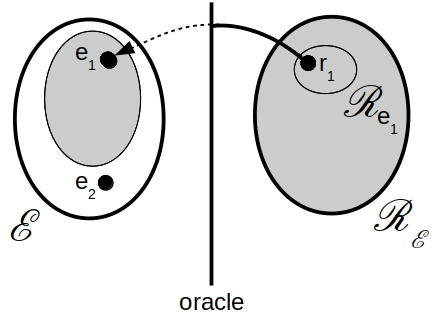
\includegraphics[scale=0.5]{entities_topics_1}
% \caption{\label{fig:entities_topics_1}Encodings and Entities.}
% \end{figure}

We distinguish between \emph{knowable} and \emph{unknowable} entities (see the gray areas in Figure~\ref{fig:entities_topics_1}; for example, the entity $e_2$ is not encoded by any string). An entity is said to be knowable if the oracle can reconstruct it from at least one decodable representation string. Knowability is therefore always relative to the particular oracle under consideration.

\begin{definition}
\label{def:knowable_entity}
We say that an entity $e \in \mathcal{E}$ is \emph{oracle knowable}\index{Oracle knowable} with respect to the oracle $\mathcal{O}_{\mathcal{E}}$ if there exists at least one $r \in \mathcal{R}_{\mathcal{O}_{\mathcal{E}}}^{\top}$ such that $\delta_\mathcal{O}(r) = e$. An entity $e \in \mathcal{E}$ is \emph{oracle unknowable}\index{Oracle unknowable} if it is not oracle knowable with respect to $\mathcal{O}_{\mathcal{E}}$.
\end{definition}

An entity that is unknowable with respect to one oracle, for example because that oracle's internal reconstruction mechanism or representation style is too weak, may become knowable with respect to another oracle that adopts a different style or has greater reconstructive capacity.

\begin{example}
Consider Example~\ref{ex:formal_languages_oracles}. The language
\[
L_1 = \{\, a^n b^n \mid n \ge 0 \,\}
\]
cannot be recognized by any finite automaton, and therefore it is not decodable under the finite-automaton representation style. However, it can be generated by a context-free grammar, and thus becomes decodable under the pushdown-automaton style.

Similarly, the language
\[
L_2 = \{\, a^n b^n c^n \mid n \ge 0 \,\}
\]
is not context-free and therefore cannot be decoded under the pushdown-automaton style, but it can be recognized by a Turing machine. Consequently, it becomes decodable under the Turing-machine representation style.
\end{example}

We are interested in the set of all those entities that are knowable, that is, the entities for which there exists at least one representation that decodes the entity.

\begin{definition}
Given a representation oracle $\mathcal{O}_{\mathcal{E}}$ over the set of entities $\mathcal{E}$, we define the set of \emph{oracle-knowable entities} by
\[
\mathcal{E}_{\mathcal{O}}^{\top} = \left\{e\in\mathcal{E} \mid
\exists r\in\mathcal{R}_{\mathcal{O}}^{\top}
\text{ such that }
\delta_{\mathcal{O}}(r)=e
\right\}.
\]
\end{definition}

The fact that representations are finite binary strings imposes an immediate cardinality constraint on oracle-mediated knowledge. Even if the oracle is idealized and non-computable, it can only decode countably many representations, and therefore can make at most countably many entities knowable.

\begin{proposition}
\label{prop:countable_oracle_knowable}
For any oracle \(\mathcal{O}_{\mathcal E}\), the set of oracle-knowable entities \(\mathcal{E}_{\mathcal O}^{\top}\) is countable.
\end{proposition}
\begin{proof}
By definition,
\[
\mathcal{E}_{\mathcal O}^{\top}
=
\{\delta_{\mathcal O}(r)\mid r\in\mathcal{R}_{\mathcal O}^{\top}\}.
\]
Since \(\mathcal{R}_{\mathcal O}^{\top}\subseteq\mathcal{B}^\ast\) and \(\mathcal{B}^\ast\) is countable, the set \(\mathcal{R}_{\mathcal O}^{\top}\) is countable. The image of a countable set under a function is countable. Therefore \(\mathcal{E}_{\mathcal O}^{\top}\) is countable.
\end{proof}

This limitation has an immediate consequence for sufficiently large domains of inquiry. If the set of entities under consideration is uncountable, then no oracle based on finite representations can make all of them knowable.

\begin{proposition}
\label{prop:uncountable_entities_unknowable}
If the set of entities \(\mathcal{E}\) is uncountable, then for any oracle \(\mathcal{O}_{\mathcal E}\),
\[
\mathcal E\setminus \mathcal{E}_{\mathcal O}^{\top}\neq\varnothing.
\]
\end{proposition}
\begin{proof}
By Proposition~\ref{prop:countable_oracle_knowable}, the set \(\mathcal{E}_{\mathcal O}^{\top}\) is countable. Since \(\mathcal E\) is uncountable, \(\mathcal{E}_{\mathcal O}^{\top}\) cannot exhaust \(\mathcal E\). Hence
\[
\mathcal E\setminus \mathcal{E}_{\mathcal O}^{\top}\neq\varnothing.
\]
\end{proof}

\begin{example}
\label{ex:unknowability_real_numbers}
Consider the case in which the entities under study are real numbers, so that \(\mathcal{E}=\mathbb{R}\).
Since the set of finite binary strings \(\mathcal{B}^\ast\) is countable, any oracle \(\mathcal{O}_{\mathcal{E}}\) can decode at most countably many representations. Consequently, the set of oracle-knowable real numbers
\[
\mathcal{E}_{\mathcal{O}}^{\top}
=
\{\,\delta_{\mathcal O}(r)\mid r\in\mathcal{R}_{\mathcal O}^{\top}\,\}
\]
is countable. Because the set of real numbers \(\mathbb{R}\) is uncountable, there must exist real numbers that cannot be reconstructed from any finite binary representation under the oracle.
\end{example}

Example~\ref{ex:unknowability_real_numbers} illustrates a fundamental limitation of representation-based knowledge. In domains where the set of possible entities is uncountable, the space of entities necessarily exceeds the space of finite representations available to us. As a consequence, even an idealized oracle cannot make all entities knowable through finite descriptions.

%
% Minimal Representations
%

\section{Minimal Representations}

Once a representation oracle $\mathcal{O}$ and the notion of decodable representation have been defined, it becomes possible to compare different representations of a given entity. In general, an entity $e \in \mathcal{E}$ may admit multiple distinct decodable representations, since different binary strings may contain sufficient information for the oracle to reconstruct the same entity. These representations may differ significantly in length, reflecting the presence of symbols that are not strictly required for reconstruction.

From a theoretical perspective, it is therefore natural to identify those representations that encode an entity in the most economical manner. Intuitively, such representations are those for which no shorter decodable representation of the same entity exists under the oracle: if a shorter representation existed that allowed the oracle to reconstruct the same entity, the longer one would not be minimal. We refer to these encodings as \emph{minimal representations}. They form one of the most stringent classes of representations in the theory of nescience, since they require shortest-length decodability for a given entity under a fixed oracle.

\begin{definition}
\label{def:nonredundant_description}
Let $\mathcal{E}$ be a set of entities, and $\mathcal{O}_\mathcal{E}$ be an oracle with reconstruction function $\delta$. We say that the decodable representation $r \in \mathcal{R}^{\top}$ is a \emph{minimal}\index{Minimal representation} representation if there is no decodable representation $s\in\mathcal{R}^{\top}$ such that
\[
l(s) < l(r) \wedge\ \delta(s) = \delta(r)
\]
We denote by $\mathcal{R}^{\star}_{\mathcal{O}_{\mathcal{E}}}$ the set of minimal representations for $\mathcal{E}$.
\end{definition}

Because the internal reconstruction mechanism of the oracle is abstract and, in general, inaccessible, it is natural to regard the oracle as a black box and to characterize it solely through its observable input/output behaviour. Within this perspective, the set of minimal representations provides a particularly informative external description of the oracle. It consists of those decodable representations that achieve minimal length for each reconstructible entity, thereby indicating both which entities the oracle can decode and the shortest forms from which they can be recovered.

\begin{notation}
When the set of entities $\mathcal{E}$ is clear from the context we write $\mathcal{R}^{\star}_{\mathcal{O}}$, and when the oracle is also clear we simply write $\mathcal{R}^{\star}$.
\end{notation}

An entity may admit multiple minimal representations, each of equal length and decodable by the oracle. It is therefore convenient to consider the collection of all minimal representations that reconstruct the same entity.

\begin{definition}
Let $\mathcal{O}$ be a representation oracle with reconstruction function $\delta : \mathcal{B}^\ast \rightharpoonup \mathcal{E}$, and let $e \in \mathcal{E}$ be an entity. We define the \emph{set of minimal representations of $e$} as
\[
\mathcal{R}^{\star}_{e} = \bigl\{r \in \mathcal{R}^{\star} \;\big|\; \delta(r)=e \bigr\}.
\]
\end{definition}

\noindent
In other words, $\mathcal{R}^{\star}_{e}$ is the set of all minimal representations that decode the entity $e$ under the oracle $\mathcal{O}$.

\begin{example}
Let $\mathcal{E}$ be a set of entities consisting of chemical compounds, and let $\mathcal{O}_{\mathcal{E}}$ be a representation oracle whose reconstruction function $\delta$ maps valid molecular encodings to their corresponding molecular structure (e.g., as a labeled graph of atoms and bonds). Assume that the oracle accepts strings written in a non-canonical linear encoding scheme in which any traversal-compatible ordering of atoms is permitted, provided that the resulting string encodes the correct connectivity. In particular, different linearizations of the same molecular graph may yield distinct valid strings. Consider the molecule ethanol, denoted by $e \in \mathcal{E}$. Under such a non-canonical encoding, the same molecule may admit multiple valid representations of equal length. For instance,
\[
r_1 = \texttt{CCO}, \qquad r_2 = \texttt{OCC}.
\]
Both strings are valid encodings under the chosen convention and satisfy
\[
\delta(r_1)=\delta(r_2)=e.
\]
Moreover, they have the same length, reflecting two different admissible linearizations of the same molecular structure. Assuming that no shorter valid encoding exists for this molecule within the given encoding scheme, both $r_1$ and $r_2$ are minimal representations of $e$, that is,
\[
r_1, r_2 \in \mathcal{R}^\star_e.
\]
\end{example} 

Before studying the properties of minimal representations, it is important to establish that such representations always exist for entities that the oracle can decode. Intuitively, if an entity admits at least one decodable representation, then among all such representations there must be one of minimal length. The following proposition formalizes this observation.

\begin{proposition}
Let $\mathcal{O}$ be a representation oracle and let $e \in \mathcal{E}$ be a oracle-knowable entity. Then there exists at least one minimal representation $r \in \mathcal{R}^{\star}_{e}$.
\end{proposition}

\begin{proof}
Since $e$ is decodable, there exists at least one representation $r_0 \in \mathcal{R}^{\top}$ such that $\delta(r_0)=e$. Hence the set
\[
A_e = \{\, l(r) : r \in \mathcal{R}^{\top},\ \delta(r)=e \,\} \subseteq \mathbb{N}
\]
is non-empty. Because $\mathbb{N}$ is well ordered, the set $A_e$ admits a minimum element, say $m$. Choose a representation $r \in \mathcal{R}^{\top}$ such that $\delta(r)=e$ and $l(r)=m$. By definition of $m$, there exists no representation $s \in \mathcal{R}^{\top}$ such that $\delta(s)=e$ and $l(s) < l(r)$. Therefore, $r$ is a minimal representation of $e$, and thus $r \in \mathcal{R}^{\star}_{e}$.
\end{proof}

This result shows that every decodable entity admits at least one minimal representation. In general, however, the minimal representation of an entity need not be unique: several distinct strings may achieve the same minimal length while still allowing the oracle to reconstruct the same entity.

\begin{example}
Let $\mathcal{E}$ be a set of entities consisting of finite undirected graphs with labeled vertices, and let $\mathcal{O}_{\mathcal{E}}$ be a representation oracle whose reconstruction function $\delta$ interprets binary strings as adjacency matrices encoded row by row. A string $r \in \mathcal{B}^\ast$ is decodable if it encodes an integer $n$ (the number of vertices) followed by $n^2$ bits specifying the adjacency matrix. The oracle ignores any additional trailing bits beyond this structure.

Consider the graph $e \in \mathcal{E}$ consisting of two vertices connected by a single edge. The following strings are all decodable representations of $e$:
\[
r_1 = [n=2][0110][0000], \;
r_2 = [n=2][0110][\text{metadata}], \;
r_3 = [n=2][0110]
\]
They satisfy $\delta(r_1)=\delta(r_2)=\delta(r_3)=e$. However, $r_1$ and $r_2$ contain additional symbols that are ignored by the reconstruction function, and therefore play no role in determining the entity. Among these representations, $r_3$ has minimal length.
\end{example}

The sets $\mathcal{R}^\star_{e}$ introduced above collect the minimal representations associated with each individual decodable entity. The next proposition shows that these sets exhaust the whole set of minimal representations: every minimal representation belongs to exactly one such class, namely, the class determined by the entity reconstructed by the oracle.

\begin{proposition}
Let $\mathcal{E}$ be a set of entities and $\mathcal{O}_\mathcal{E}$ be a representation oracle with reconstruction function $\delta$. We have that
\[
\mathcal{R}^{\star}_{\mathcal{O}_\mathcal{E}} = \bigcup_{e \in \mathcal{E}_{\mathcal{O}}^{\top}}\mathcal{R}^{\star}_{e}.
\]
\end{proposition}
\begin{proof}
First, let $r \in \mathcal{R}^{\star}_{\mathcal{O}_\mathcal{E}}$. Since $r$ is a minimal representation, it is in particular decodable, so $\delta(r)$ is defined. Let $e=\delta(r)$. Then $e\in\mathcal{E}_{\mathcal{O}}^{\top}$ by definition of knowable entity. Moreover, since $r \in \mathcal{R}^{\star}$ and $\delta(r)=e$, the definition of $\mathcal{R}^{\star}_{e}$ gives $r \in \mathcal{R}^{\star}_{e}$. Hence
\[
r\in \bigcup_{e\in\mathcal{E}_{\mathcal{O}}^{\top}}\mathcal{R}^{\star}_{e},
\]
and therefore
\[
\mathcal{R}^{\star}_{\mathcal{O}_\mathcal{E}} \subseteq \bigcup_{e\in\mathcal{E}_{\mathcal{O}}^{\top}}\mathcal{R}^{\star}_{e}.
\]
Conversely, let
\[
r\in \bigcup_{e\in\mathcal{E}_{\mathcal{O}}^{\top}}\mathcal{R}^{\star}_{e}.
\]
Then there exists some $e \in \mathcal{E}_{\mathcal{O}}^{\top}$ such that $r\in\mathcal{R}^{\star}_{e}$. By definition of $\mathcal{R}^{\star}_{e}$, this means that $r\in\mathcal{R}^{\star}_{\mathcal{O}_\mathcal{E}}$ and $\delta(r)=e$. In particular, $r\in\mathcal{R}^{\star}$. Therefore
\[
\bigcup_{e\in\mathcal{E}_{\mathcal{O}}^{\top}}\mathcal{R}^{\star}_{e}\subseteq \mathcal{R}^{\star}_{\mathcal{O}_\mathcal{E}}.
\]
\end{proof}

Minimal representations correspond to entities through the reconstruction function of the oracle. It is therefore natural to ask whether a single minimal representation could correspond to more than one entity. The following proposition shows that this cannot occur: the sets of minimal representations associated with different entities are disjoint.

\begin{proposition}
Let $e_1,e_2 \in \mathcal{E}$ with $e_1 \neq e_2$. Then
\[
\mathcal{R}^\star_{e_1} \cap \mathcal{R}^\star_{e_2} = \varnothing .
\]
\end{proposition}
\begin{proof}
Suppose, for contradiction, that there exists a string $r \in \mathcal{R}^\star_{e_1} \cap \mathcal{R}^\star_{e_2}$. By definition of $\mathcal{R}^\star_{e_1}$ we have that $\delta(r)=e_1$, and by definition of $\mathcal{R}^\star_{e_2}$ we have $\delta(r)=e_2$. Since $\delta$ is a function on its domain, it assigns a unique value to each $r \in \mathcal{B}^\ast$ for which it is defined. Hence $e_1=e_2$, contradicting the assumption that $e_1 \neq e_2$.
\end{proof}

This proposition shows that the sets $\mathcal{R}^\star_{e}$ form a collection of pairwise disjoint subsets of $\mathcal{R}^\star$. Consequently, each minimal representation identifies a unique entity under the oracle, and the reconstruction function $\delta$ induces a natural partition of the set of minimal representations according to the entities they encode.

A natural question is whether the notion of minimal representation depends on the particular coding scheme used to write representations as binary strings. The following proposition shows that minimality is invariant under any computable bijection that merely renames representations without altering their lengths. In this sense, minimal representations are stable under effective recodings of fixed size.

\begin{proposition}
Let $\mathcal{O}_{\mathcal{E}}$ be a representation oracle with reconstruction function $\delta_{\mathcal{O}}$, and let $f:\mathcal{B}^\ast \to \mathcal{B}^\ast$ be a total computable bijection such
that
\[
l(f(x)) = l(x)
\qquad
\text{for all } x \in \mathcal{B}^\ast.
\]
Define the transported reconstruction function
\[
\delta'_{\mathcal{O}}(x) := \delta_{\mathcal{O}}(f^{-1}(x)).
\]
Let $\mathcal{R}^\star_{\mathcal{O}_{\mathcal{E}}}$ be the set of minimal representations induced by $\delta_{\mathcal{O}}$, and let $\mathcal{R}^\star_{\mathcal{O}'_{\mathcal{E}}}$ be the corresponding set induced by $\delta'_{\mathcal{E}}$. Then, for every $r \in \mathcal{B}^\ast$,
\[
r \in \mathcal{R}^\star_{\mathcal{O}_{\mathcal{E}}}
\quad\Longleftrightarrow\quad
f(r) \in \mathcal{R}^\star_{\mathcal{O}'_{\mathcal{E}}}.
\]
\end{proposition}
\begin{proof}
Fix $r \in \mathcal{B}^\ast$.

First observe that decodability is preserved by $f$. Indeed, by definition of
$\delta'_{\mathcal{E}}$,
\[
\delta'_{\mathcal{E}}(f(r))
=
\delta_{\mathcal{O}}(f^{-1}(f(r)))
=
\delta_{\mathcal{O}}(r).
\]
Hence $\delta_{\mathcal{O}}(r)$ is defined if and only if $\delta'_{\mathcal{E}}(f(r))$ is defined, and in that case both reconstruct the same entity.

Assume first that
\[
r \in \mathcal{R}^\star_{\mathcal{O}_{\mathcal{E}}}.
\]
Then $r$ is a minimal representation, so $\delta_{\mathcal{O}}(r)$ is defined and there exists no decodable representation $s \in \mathcal{B}^\ast$ such
that
\[
l(s) < l(r)
\qquad\text{and}\qquad
\delta_{\mathcal{O}}(s)=\delta_{\mathcal{O}}(r).
\]
Suppose, for contradiction, that $f(r)$ is not minimal with respect to $\delta'_{\mathcal{E}}$. Then there exists some $t \in \mathcal{B}^\ast$ such that
\[
l(t) < l(f(r))
\qquad\text{and}\qquad
\delta'_{\mathcal{E}}(t)=\delta'_{\mathcal{E}}(f(r)).
\]
Let $s=f^{-1}(t)$. Since $f$ is a bijection, $s \in \mathcal{B}^\ast$, and by the length-preserving property,
\[
l(s)=l(f(s))=l(t)<l(f(r))=l(r).
\]
Moreover,
\[
\delta_{\mathcal{O}}(s)
=
\delta_{\mathcal{O}}(f^{-1}(t))
=
\delta'_{\mathcal{E}}(t)
=
\delta'_{\mathcal{E}}(f(r))
=
\delta_{\mathcal{O}}(r).
\]
Thus $s$ is a shorter decodable representation of the same entity as $r$, contradicting the minimality of $r$. Therefore $f(r)$ is minimal with respect to $\delta'_{\mathcal{E}}$.

Conversely, assume that
\[
f(r) \in \mathcal{R}^\star_{\mathcal{O}'_{\mathcal{E}}}.
\]
By the same argument applied to the bijection $f^{-1}$, which is also total, computable, bijective, and length-preserving, it follows that $r$ is minimal with respect to $\delta_{\mathcal{O}}$.

Hence
\[
r \in \mathcal{R}^\star_{\mathcal{O}_{\mathcal{E}}}
\quad\Longleftrightarrow\quad
f(r) \in \mathcal{R}^\star_{\mathcal{O}'_{\mathcal{E}}}.
\]
\end{proof}

This proposition shows that minimality is not tied to a particular binary coding, but only to the reconstruction structure induced by the oracle and to the relative lengths of equivalent encodings. In particular, any effective relabeling that preserves length leaves the class of minimal representations unchanged up to the induced bijection.

Finally, it is useful to isolate the smallest amount of algorithmic information that any decodable representation of $e$ must contain. This quantity provides a lower bound on the irreducible descriptive complexity of the entity relative to the decodability criterion.

\begin{definition}
\label{def:representational_complexity_floor}
Let $e \in \mathcal{E}_{\mathcal O}^{\top}$ be an entity and $\mathcal{O}_\mathcal{E}$ be a representational oracle. We define the \emph{representational complexity floor} of $e$ given the oracle $\mathcal{O}_\mathcal{E}$ as
\[
\kappa_e = \min_{r \in \mathcal{R}_{e}^{\top}} K(r).
\]
\end{definition}

The representational complexity floor measures the least Kolmogorov complexity among all decodable representations of $e$. In this sense, it captures the minimum amount of algorithmic information required to represent $e$.

%
% Section: Minimal Oracles
%

\section{Minimal Oracles}
\label{sec:minimal_oracles}

Ideally, representation oracles should be minimal in size, meaning that all information needed to reconstruct an entity is carried by the representation string rather than being hard-wired into the oracle. A non-minimal oracle\index{Non-minimal oracle} can simplify the representation problem by offloading complexity to its internal representation function, but it also forces researchers to understand not only the representation itself but the oracle's internal reconstruction process, something that, given the abstract nature of oracles, is generally not accessible in practice.

\begin{definition}
Let $\mathcal{O}_A$ and $\mathcal{O}_B$ be two oracles defined over the set of entities $\mathcal{E}$. We say are said that the oracles $\mathcal{O}_A$ and $\mathcal{O}_B$ are \emph{comparable}\index{Comparable oracle}, denoted by $\mathcal O_A \sim \mathcal O_B$, if
\[
\mathcal{E}_{\mathcal{O}_{A}}^{\top} = \mathcal{E}_{\mathcal{O}_{B}}^{\top}.
\]
\end{definition}

The comparability relation defined above does more than merely identify pairs of oracles with the same knowable-entity set: it partitions the entire class $\mathfrak O_{\mathcal E}$ into structurally homogeneous blocks. Within each block, all oracles agree on which entities are decodable, and differ only in how those entities are represented or reconstructed.

\begin{proposition}
The relation \(\sim\) is an equivalence relation on \(\mathfrak O_{\mathcal E}\).
\end{proposition}
\begin{proof}
Reflexivity is immediate since \(\mathcal E^{\top}_{\mathcal O}=\mathcal E^{\top}_{\mathcal O}\).
Symmetry holds because equality is symmetric.
Transitivity holds because if \(\mathcal E^{\top}_{\mathcal O_A}=\mathcal E^{\top}_{\mathcal O_B}\) and
\(\mathcal E^{\top}_{\mathcal O_B}=\mathcal E^{\top}_{\mathcal O_C}\), then
\(\mathcal E^{\top}_{\mathcal O_A}=\mathcal E^{\top}_{\mathcal O_C}\).
\end{proof}

The equivalence relation $\sim$ partitions the space of oracles into disjoint classes, each class collecting all oracles that make exactly the same entities decodable. The comparability class of an oracle thus isolates differences in representation mechanisms and internal structure while holding fixed the underlying set of decodable entities. 

\begin{definition}
Let $\mathcal O \in \mathfrak O_{\mathcal E}$ be an oracle. We define the comparability class of $\mathcal O$, denoted by $[\mathcal{O}]$, as follows:
\[
[\mathcal O] = \{\mathcal O'\in\mathfrak O_{\mathcal E}\mid \mathcal O'\sim \mathcal O\}
\]
\end{definition}

When an oracle contains hard-wired information, it can reconstruct an entity from a representation that leaves part of that information implicit, representations that an oracle without that hard-wired knowledge would be unable to decode. This property provides a natural basis for ordering oracles: we compare the sets of distinct minimal representations they accept, since an oracle with more hard-wired information admits a larger set of minimal decodable representations.

\begin{definition}
Let $\mathcal{O}_A$ and $\mathcal{O}_B$ be two comparable oracles. We say that $\mathcal{O}_A$ \emph{reduces}\index{Oracle reduction} to $\mathcal{O}_B$, denoted by $\mathcal{O}_A \triangleright \mathcal{O}_B$, if
\[
\left(
\forall e \in \mathcal{E}^\top_{\mathcal{O}_A},\;
\mathcal{R}^\star_{\mathcal{O}_B, e} \subseteq \mathcal{R}^\star_{\mathcal{O}_A, e}
\right)
\;\wedge\;
\left(
\exists e \in \mathcal{E}^\top_{\mathcal{O}_A},\;
\mathcal{R}^\star_{\mathcal{O}_B, e} \subsetneq \mathcal{R}^\star_{\mathcal{O}_A, e}
\right).
\]
\end{definition}

\noindent
An oracle is less minimal only when its internal knowledge makes it possible to reconstruct an entity from a strictly shorter encoding that omits information which another comparable oracle would require explicitly.

\begin{example}
Consider representations of chemical compounds. A non-minimal oracle may incorporate extensive background chemical knowledge (e.g., periodic table, standard valences, and common structures). Under such an oracle, a compound could be represented by a short string such as its common name (e.g., \emph{water}, \emph{ethanol}), from which the oracle reconstructs the full molecular structure. In this case, most of the information required for reconstruction is implicit in the oracle rather than explicit in the representation. By contrast, a more minimal oracle requires the representation to encode the relevant structure directly, for instance by specifying atoms and bonds.
\end{example}

The binary relation of reduction defines a non-strict partial order over the sets of all comparble oracles as next proposition shows.

\begin{proposition}
Let $\mathfrak{O}_{\mathcal{E}}$ be the set of comparable oracles over the set of entities $\mathcal{E}$. We have that the reduction relation $\triangleright$ is:
\begin{enumerate}
\item \emph{irreflexive}: $\neg(\mathcal{O} \triangleright \mathcal{O})$ for all $\mathcal{O} \in \mathfrak{O}_{\mathcal{E}}$,
\item \emph{transitive}: if $\mathcal{O}_A \triangleright \mathcal{O}_B$ and $\mathcal{O}_B \triangleright \mathcal{O}_C$, then $\mathcal{O}_A \triangleright \mathcal{O}_C$, for all $\mathcal{O}_A, \mathcal{O}_B, \mathcal{O}_C \in \mathfrak{O}_{\mathcal{E}}$
\end{enumerate}
\end{proposition}
\begin{proof}
Irreflexivity follows from the fact that no set is a strict subset of itself. Transitivity follows from transitivity of strict set inclusion.
\end{proof}

While the relation $\triangleright$ is transitive and irreflexive, it is natural to ask whether it induces a total ordering on the class of comparable oracles. The following proposition shows that this is not the case: even when two oracles decode exactly the same entities, they may embody different and incomparable forms of hard-wired information.

\begin{proposition}
It is not the case that the reduction relation \(\triangleright\) is total on
\(\mathfrak{O}_{\mathcal{E}}\).
That is, there exist comparable oracles
\(\mathcal{O}_A,\mathcal{O}_B\in\mathfrak{O}_{\mathcal{E}}\) such that neither
\(\mathcal{O}_A \triangleright \mathcal{O}_B\) nor
\(\mathcal{O}_B \triangleright \mathcal{O}_A\) holds.
\end{proposition}
\begin{proof}
We exhibit two comparable oracles whose sets of minimal representations are
incomparable under strict inclusion.

Let \(\mathcal{E}=\{e_0,e_1,e_2\}\) and fix an alphabet \(\mathcal{B}\) containing distinct symbols
\(a,b,c\).
Define two reconstruction functions
\(\delta_A,\delta_B:\mathcal{B}^\ast\rightharpoonup\mathcal{E}\) by specifying their
(minimal) decodable representations as follows:
\[
\delta_A(a)=e_0,\quad \delta_A(b)=e_1,\quad \delta_A(cc)=e_2,
\]
\[
\delta_B(aa)=e_0,\quad \delta_B(b)=e_1,\quad \delta_B(c)=e_2,
\]
and leave both functions undefined on all other strings.
Let \(\mathcal{O}_A\) and \(\mathcal{O}_B\) be the corresponding representation oracles.

By construction, both oracles decode exactly the same set of entities \(\mathcal{E}\), and hence
\(\mathcal{O}_A,\mathcal{O}_B\in\mathfrak{O}_{\mathcal{E}}\).
Moreover, their sets of minimal representations are
\[
\mathcal{R}^{\star,0}_{\mathcal{O}_A}=\{a,b,cc\},
\qquad
\mathcal{R}^{\star,0}_{\mathcal{O}_B}=\{aa,b,c\}.
\]

These two sets are incomparable under strict inclusion: we have
\(cc\in\mathcal{R}^{\star,0}_{\mathcal{O}_A}\) but
\(cc\notin\mathcal{R}^{\star,0}_{\mathcal{O}_B}\), and also
\(c\in\mathcal{R}^{\star,0}_{\mathcal{O}_B}\) but
\(c\notin\mathcal{R}^{\star,0}_{\mathcal{O}_A}\).
Therefore neither
\(\mathcal{R}^{\star,0}_{\mathcal{O}_B}\subsetneq \mathcal{R}^{\star,0}_{\mathcal{O}_A}\) nor
\(\mathcal{R}^{\star,0}_{\mathcal{O}_A}\subsetneq \mathcal{R}^{\star,0}_{\mathcal{O}_B}\) holds.

By definition of the reduction relation \(\triangleright\), this implies that neither
\(\mathcal{O}_A \triangleright \mathcal{O}_B\) nor
\(\mathcal{O}_B \triangleright \mathcal{O}_A\) holds.
Hence \(\triangleright\) is not a total relation on \(\mathfrak{O}_{\mathcal{E}}\).
\end{proof}

This proposition shows that even when the set of knowable entities is held fixed, there may be multiple, genuinely different ways of distributing information between representations and the oracle.
Different oracles may hard-wire different aspects of the same entities, leading to incomparable minimal representation sets. As a consequence, simplification with respect to \(\triangleright\) is not a linear process but a partial ordering, and minimal oracles, when they exist, need not be unique.

The ordering introduced by the reduction relation allow us to formally introduce the concept of minimality: an oracle is minimal if it cannot be reduced to any other comparable oracle.

\begin{definition}
\label{def:minimal_oracle}
Let $\mathcal{O} \in \mathfrak{O}_{\mathcal{E}}$ be an oracle. We say that $\mathcal{O}$ is \emph{minimal}\index{Minimal oracle} if
\[
\nexists \mathcal{O}' \in [\mathcal{O}] : \mathcal{O} \triangleright \mathcal{O}'.
\]
\end{definition}

\noindent
Equivalently, the oracle $\mathcal{O}$ is minimal if there is no $\mathcal{O}' \in [\mathcal{O}]$ such that
\[
\left(
\forall e \in \mathcal{E}^\top_{\mathcal{O}},\;
\mathcal{R}^\star_{\mathcal{O}', e} \subseteq \mathcal{R}^\star_{\mathcal{O}, e}
\right)
\;\wedge\;
\left(
\exists e \in \mathcal{E}^\top_{\mathcal{O}},\;
\mathcal{R}^\star_{\mathcal{O}', e} \subsetneq \mathcal{R}^\star_{\mathcal{O}, e}
\right).
\]

The notion of minimal oracle formalizes the idea of an oracle that contains no unnecessary hard-wired information relative to a fixed representation style and a fixed set of knowable entities. Recall that a reduction $\mathcal{O}\triangleright\mathcal{O}'$ corresponds to eliminating part of the oracle's internalized assumptions while preserving the same epistemic reach, a change that is reflected in a strict reduction of the set of minimal decodable representations. An oracle is therefore minimal precisely when no further such elimination is possible within its comparability class.

This does not mean that a minimal oracle is devoid of internal structure or background knowledge; rather, it means that any remaining hard-wired information is irreducible given the chosen representation style.
In this sense, minimal oracles capture the simplest reconstruction mechanisms compatible with that style, and they formalize the intuition of oracles that do not rely on avoidable internalized assumptions.

\begin{definition}
\label{def:class_minimal_oracles}
Let $\mathcal{E}$ be a set of entities and let $\mathfrak{O}_{\mathcal{E}}$ be the class of representation oracles over $\mathcal{E}$. We define the set of \emph{minimal oracles}\index{Minimal oracle} as
\[
\mathfrak{O}_{\mathcal{E}}^{\min}
\;=\;
\left\{
\mathcal{O} \in \mathfrak{O}_{\mathcal{E}}
\;\middle|\;
\nexists \mathcal{O}' \in [\mathcal{O}] \text{ such that } \mathcal{O} \triangleright \mathcal{O}'
\right\}.
\]
\end{definition}

The class $\mathfrak{O}_{\mathcal{E}}^{\min}$ collects those oracles that are minimal with respect to the reduction relation within their comparability class.

The following proposition provides an alternative characterization of minimal oracles in terms of minimal elements under pointwise set inclusion.

\begin{proposition}
\label{prop:characterization_minimality}
Let $\mathcal{E}$ be a set of entities and let $\mathcal{O} \in \mathfrak{O}_{\mathcal{E}}$. Then $\mathcal{O}$ is minimal if and only if the family
\[
\bigl\{\mathcal{R}^\star_{\mathcal{O}, e}\bigr\}_{e \in \mathcal{E}^\top_{\mathcal{O}}}
\]
is a minimal element, under pointwise set inclusion, among the families
\[
\left\{
\bigl\{\mathcal{R}^\star_{\mathcal{O}', e}\bigr\}_{e \in \mathcal{E}^\top_{\mathcal{O}}}
:\;
\mathcal{O}' \in [\mathcal{O}]
\right\}.
\]
\end{proposition}

\begin{proof}
By Definition~\ref{def:minimal_oracle}, the oracle $\mathcal{O}$ is minimal if and only if there is no $\mathcal{O}' \in [\mathcal{O}]$ such that $\mathcal{O} \triangleright \mathcal{O}'$. By the definition of the reduction relation, this is equivalent to the non-existence of $\mathcal{O}' \in [\mathcal{O}]$ such that
\[
\left(
\forall e \in \mathcal{E}^\top_{\mathcal{O}},\;
\mathcal{R}^\star_{\mathcal{O}', e} \subseteq \mathcal{R}^\star_{\mathcal{O}, e}
\right)
\;\wedge\;
\left(
\exists e \in \mathcal{E}^\top_{\mathcal{O}},\;
\mathcal{R}^\star_{\mathcal{O}', e} \subsetneq \mathcal{R}^\star_{\mathcal{O}, e}
\right).
\]
This condition is precisely the statement that the family $\{\mathcal{R}^\star_{\mathcal{O}, e}\}_{e \in \mathcal{E}^\top_{\mathcal{O}}}$ is minimal under pointwise set inclusion among the corresponding families induced by oracles in $[\mathcal{O}]$.
\end{proof}

Minimal oracles need not be unique. It may happen that two distinct oracles $\mathcal{O}_A, \mathcal{O}_B \in \mathfrak{O}_{\mathcal{E}}$ are both minimal, while their sets of minimal representations $\mathcal{R}^\star_{\mathcal{O}_A}$ and $\mathcal{R}^\star_{\mathcal{O}_B}$ are incomparable under set inclusion. In such a case, neither oracle can be reduced to the other, and both appear as minimal elements of the partial order induced by the reduction relation.

The existence of minimal oracles depends on the size of the subset of decodable entities and on the amount of freedom allowed in the representation mechanism.

\begin{proposition}
\label{prop:existence_minimal_finite}
Let $\mathcal{O} \in \mathfrak{O}_{\mathcal{E}}$ and let $S := \mathcal{E}^\top_{\mathcal{O}}$ be finite. Then there exists at least one minimal oracle in the comparability class $[\mathcal{O}]$ with respect to the reduction relation $\triangleright$.
\end{proposition}

\begin{proof}
Fix $\mathcal{O}' \in [\mathcal{O}]$ and $e \in S$. By definition of minimal representations,
\[
\mathcal{R}^\star_{\mathcal{O}', e}
=
\{\, r \in \mathcal{R}^\top_{\mathcal{O}'} : \delta_{\mathcal{O}'}(r)=e,\; l(r)=L_{\mathcal{O}'}(e) \,\},
\]
where
\[
L_{\mathcal{O}'}(e)
=
\min \{\, l(r) : \delta_{\mathcal{O}'}(r)=e \,\}.
\]
Hence $\mathcal{R}^\star_{\mathcal{O}', e} \subseteq \mathcal{B}^{L_{\mathcal{O}'}(e)}$, and therefore $\mathcal{R}^\star_{\mathcal{O}', e}$ is finite.

Since $S$ is finite, the family
\[
\bigl\{ \mathcal{R}^\star_{\mathcal{O}', e} \bigr\}_{e \in S}
\]
consists of finitely many finite sets.

Consider the collection
\[
\mathcal{F}
:=
\left\{
\bigl\{ \mathcal{R}^\star_{\mathcal{O}', e} \bigr\}_{e \in S}
:\;
\mathcal{O}' \in [\mathcal{O}]
\right\}
\]
ordered by the strict pointwise relation induced by $\triangleright$, that is,
\[
\bigl\{A_e\bigr\}_{e \in S} \prec \bigl\{B_e\bigr\}_{e \in S}
\;\Longleftrightarrow\;
\left(
\forall e \in S,\; A_e \subseteq B_e
\right)
\wedge
\left(
\exists e \in S,\; A_e \subsetneq B_e
\right).
\]

We claim that there is no infinite strictly descending chain in $\mathcal{F}$ under $\prec$. Indeed, for each family $\{A_e\}_{e \in S}$ define the measure
\[
\mu(\{A_e\}_{e \in S}) := \sum_{e \in S} |A_e|.
\]
Each strict step $\{A_e\} \succ \{B_e\}$ decreases $\mu$ by at least one, since there exists some $e$ with $B_e \subsetneq A_e$. As $\mu$ takes values in $\mathbb{N}$, no infinite strictly descending chain exists.

Therefore, $\mathcal{F}$ admits at least one minimal element. Let
\[
\bigl\{ \mathcal{R}^\star_{\mathcal{O}^\ast, e} \bigr\}_{e \in S}
\]
be such a minimal element. By construction, there is no $\mathcal{O}' \in [\mathcal{O}]$ such that $\mathcal{O}^\ast \triangleright \mathcal{O}'$. Hence $\mathcal{O}^\ast$ is minimal.
\end{proof}

When the set of decodable entities is infinite, minimality is no longer guaranteed. Even though each individual entity $e\in S$ still admits at least one minimal representation, an oracle may allow multiple minimal representations for infinitely many entities. In that situation, one can construct an infinite strictly descending chain of oracles by successively removing some of these additional minimal representations while preserving at least one minimal representation for every entity.

\begin{proposition}
\label{prop:nonexistence_minimal_infinite}
It is not the case that, for every infinite set of entities $S \subseteq \mathcal{E}$, the comparability class of oracles decoding $S$ contains a $\triangleright$-minimal oracle.
\end{proposition}

\begin{proof}
Let $S=\{e_1, e_2, e_3, \dots\}$ be an infinite set of entities. For each $n \ge 1$, define an oracle $\mathcal{O}_n$ with reconstruction function $\delta_n:\mathcal{B}^\ast\rightharpoonup S$ by setting, for every $k \ge 1$,
\[
\delta_n(1^k)=e_k,
\qquad
\delta_n(0^{k-1}1)=e_k \quad \text{for all } k\ge n,
\]
and leaving $\delta_n(r)$ undefined for all other strings $r$.

By construction, each oracle $\mathcal{O}_n$ decodes exactly the set $S$, and therefore all $\mathcal{O}_n$ belong to the same comparability class.

For each $k \ge 1$, the shortest length of a decodable representation of $e_k$ under $\mathcal{O}_n$ is $k$, since $\delta_n(1^k)=e_k$ and no shorter string decodes to $e_k$. Hence,
\[
\mathcal{R}^\star_{\mathcal{O}_n, e_k}
=
\begin{cases}
\{\,1^k\,\}, & k < n,\\[4pt]
\{\,1^k,\;0^{k-1}1\,\}, & k \ge n.
\end{cases}
\]

Fix $n \ge 1$. Then for every $k \ge 1$ we have
\[
\mathcal{R}^\star_{\mathcal{O}_{n+1}, e_k}
\subseteq
\mathcal{R}^\star_{\mathcal{O}_n, e_k},
\]
and for $k=n$ the inclusion is strict:
\[
\mathcal{R}^\star_{\mathcal{O}_{n+1}, e_n}
=
\{\,1^n\,\}
\subsetneq
\{\,1^n,\;0^{n-1}1\,\}
=
\mathcal{R}^\star_{\mathcal{O}_n, e_n}.
\]
Therefore,
\[
\mathcal{O}_n \triangleright \mathcal{O}_{n+1}
\quad \text{for all } n \ge 1.
\]

This yields an infinite strictly descending chain
\[
\mathcal{O}_1 \triangleright \mathcal{O}_2 \triangleright \mathcal{O}_3 \triangleright \cdots.
\]
Consequently, no oracle in this family is minimal with respect to $\triangleright$.
\end{proof}

The previous proposition shows that minimal oracles need not exist when the set of decodable entities is infinite. The obstruction arises when an oracle admits additional minimal representations for infinitely many entities, making it possible to construct an infinite strictly descending chain under the reduction relation. The next proposition gives a simple sufficient condition ensuring existence: if, within a comparability class, the total number of additional minimal representations beyond one per entity is always finite, then at least one minimal oracle must exist.

\begin{proposition}
\label{prop:existence_minimal_infinite_sufficient}
Let $\mathcal{O} \in \mathfrak{O}_{\mathcal{E}}$, and let $S:=\mathcal{E}^{\top}_{\mathcal{O}}$, which may be infinite. Assume that for every oracle $\mathcal{O}' \in [\mathcal{O}]$, the quantity
\[
\mu(\mathcal{O}')
\;:=\;
\sum_{e\in S} \bigl(|\mathcal{R}^{\star}_{\mathcal{O}',e}|-1\bigr)
\]
is finite. Then there exists at least one minimal oracle in the comparability class $[\mathcal{O}]$ with respect to the reduction relation $\triangleright$.
\end{proposition}

\begin{proof}
Since $\mathcal{O}\in[\mathcal{O}]$, the comparability class $[\mathcal{O}]$ is nonempty. By hypothesis, for every $\mathcal{O}'\in[\mathcal{O}]$, the value $\mu(\mathcal{O}')$ is a finite natural number. Therefore the set
\[
M
:=
\{\mu(\mathcal{O}') : \mathcal{O}'\in[\mathcal{O}]\}
\subseteq \mathbb{N}
\]
is nonempty, and hence admits a least element. Choose an oracle $\mathcal{O}^{\ast}\in[\mathcal{O}]$ such that
\[
\mu(\mathcal{O}^{\ast})=\min M.
\]

We claim that $\mathcal{O}^{\ast}$ is minimal. Suppose, for contradiction, that it is not. Then there exists an oracle $\mathcal{O}'\in[\mathcal{O}]$ such that
\[
\mathcal{O}^{\ast}\triangleright \mathcal{O}'.
\]
By definition of the reduction relation, this means that
\[
\forall e\in S,\qquad
\mathcal{R}^{\star}_{\mathcal{O}',e}\subseteq \mathcal{R}^{\star}_{\mathcal{O}^{\ast},e},
\]
and
\[
\exists e_{0}\in S,\qquad
\mathcal{R}^{\star}_{\mathcal{O}',e_{0}}\subsetneq \mathcal{R}^{\star}_{\mathcal{O}^{\ast},e_{0}}.
\]

Since strict inclusion of finite sets strictly decreases cardinality, we obtain
\[
|\mathcal{R}^{\star}_{\mathcal{O}',e}|
\le
|\mathcal{R}^{\star}_{\mathcal{O}^{\ast},e}|
\qquad\forall e\in S,
\]
and
\[
|\mathcal{R}^{\star}_{\mathcal{O}',e_{0}}|
<
|\mathcal{R}^{\star}_{\mathcal{O}^{\ast},e_{0}}|.
\]
Subtracting $1$ from each side preserves these inequalities, so
\[
|\mathcal{R}^{\star}_{\mathcal{O}',e}|-1
\le
|\mathcal{R}^{\star}_{\mathcal{O}^{\ast},e}|-1
\qquad\forall e\in S,
\]
with strict inequality for $e=e_{0}$. Summing over all $e\in S$, and using the finiteness of both sums, yields
\[
\mu(\mathcal{O}')
<
\mu(\mathcal{O}^{\ast}),
\]
contradicting the minimality of $\mu(\mathcal{O}^{\ast})$.

Therefore no such oracle $\mathcal{O}'$ exists, and $\mathcal{O}^{\ast}$ is minimal.
\end{proof}

This proposition shows that the failure of minimality in the infinite case is not caused merely by the infinitude of the decodable set. What matters is whether the comparability class contains an unbounded supply of removable minimal representations. If the total excess of minimal representations remains finite for every oracle in the class, then the reduction process cannot continue indefinitely, and a minimal oracle must exist.

In some domains with composed by an infinite collection of entities, such as mathematics, scientific knowledge can exhibit a form of unbounded refinement. As inquiry progresses and finer distinctions become relevant, representations may need to become increasingly detailed (and thus longer), while at the same time the set of admissible minimal representations becomes more constrained. In such settings there may be no final, irreducible level of representation, so minimality should be understood as a limiting ideal rather than a reachable endpoint.

\begin{example}
A paradigmatic example of an entity that requires infinite refinement of its representations is
Chaitin's halting probability \(\Omega\).
Fix a universal prefix-free Turing machine \(U\), and define
\[
\Omega \;=\; \sum_{p \text{ halts}} 2^{-|p|},
\]
where the sum ranges over all binary programs \(p\) that halt on \(U\).
The number \(\Omega\) is a well-defined real number in \((0,1)\), but it is known to be non-computable and algorithmically random.
In the present framework, \(\Omega\) may be included as an entity \(e_\Omega \in \mathcal{E}\), but its reconstruction places extreme demands on representations.

Consider a representation style in which representations are finite binary strings encoding partial information about \(\Omega\), for example its first \(n\) binary digits.
A minimal oracle \(\mathcal{O}_{\mathcal{E}}\) operating under this style does not contain any hard-wired information about the halting behavior of programs; it can only reconstruct what is explicitly provided by the string.
For each \(n\), there exist representations \(r_n \in \mathcal{B}^\ast\) such that \(\delta_{\mathcal{O}}(r_n)\) corresponds to an \(n\)-bit approximation of \(\Omega\), but no finite string \(r\) allows the oracle to reconstruct \(\Omega\) exactly.
Any improvement in accuracy requires a strictly longer representation, yielding an infinite chain
\[
r_1 \prec r_2 \prec r_3 \prec \cdots
\]
of minimal representations, with no maximal element.

The case of \(\Omega\) illustrates a situation in which an entity is, in principle, part of scientific or mathematical discourse, yet resists complete reconstruction under any minimal oracle constrained to finite representations.
Knowledge of \(\Omega\) advances only through unbounded refinement: each additional bit of information requires new, irreducible representational content.
In this sense, \(\Omega\) exemplifies an entity for which minimality is attainable only as a limiting ideal, not as a concrete endpoint, and it sharply delineates the boundary between infinite refinement of representations and full oracle-relative knowability.
\end{example}

The non-existence of minimal oracles in open-ended domains should not be interpreted as a limitation of scientific inquiry, but as an expression of its inherently exploratory character: progress consists in successive local refinements rather than in convergence to a final, irreducible description.

A natural question is whether there exists a single best oracle, in the sense of decoding every entity that is decodable under some oracle. If such an oracle existed, one could fix it once and for all and declare an entity knowable precisely when it is decodable with respect to it. The following theorem shows that this is not the case in general.

\begin{theorem}
\label{thm:no_maximal_oracle}
Let $\mathcal{E}$ be a set of entities and let $\mathfrak{O}_{\mathcal{E}}$ be the class of representation oracles over $\mathcal{E}$. Then it is not the case that $\mathfrak{O}_{\mathcal{E}}$ always contains an oracle $\mathcal{O}^{\max}$ such that
\[
\mathcal{E}^{\top}_{\mathcal{O}}
\subseteq
\mathcal{E}^{\top}_{\mathcal{O}^{\max}}
\qquad
\forall \mathcal{O} \in \mathfrak{O}_{\mathcal{E}},
\]
and $\mathcal{O}^{\max}$ is minimal in its comparability class $[\mathcal{O}^{\max}]$.
\end{theorem}

\begin{proof}
We construct a family of oracles with mutually incompatible representation styles.

Let $\mathcal{E}=\{e_1,e_2,e_3,\dots\}$ be a countable set of entities. For each $i\ge 1$, define an oracle $\mathcal{O}_i$ with reconstruction function $\delta_i:\mathcal{B}^\ast \rightharpoonup \mathcal{E}$ as follows:
\[
\delta_i(i^k)=e_k \quad \text{for all } k\ge 1,
\]
and leave $\delta_i(r)$ undefined for all other strings $r$.

Each oracle $\mathcal{O}_i$ decodes the same set of entities,
\[
\mathcal{E}^\top_{\mathcal{O}_i} = \mathcal{E},
\]
but uses a distinct encoding convention based on repetitions of the symbol $i$.

Now suppose, for contradiction, that there exists an oracle $\mathcal{O}^{\max}\in\mathfrak{O}_{\mathcal{E}}$ such that
\[
\mathcal{E}^\top_{\mathcal{O}_i} \subseteq \mathcal{E}^\top_{\mathcal{O}^{\max}}
\qquad \forall i\ge 1,
\]
and that $\mathcal{O}^{\max}$ is minimal in its comparability class.

Since each $\mathcal{O}_i$ decodes all entities in $\mathcal{E}$, the oracle $\mathcal{O}^{\max}$ must decode every $e_k$ from some representation. In particular, for each $i$ and each $k$, there must exist a string $r_{i,k}$ such that
\[
\delta_{\mathcal{O}^{\max}}(r_{i,k}) = e_k.
\]

However, the encodings used by different oracles $\mathcal{O}_i$ are mutually incompatible: the strings $i^k$ carry no information about the encoding scheme used by $j^k$ for $j\neq i$. In order for $\mathcal{O}^{\max}$ to decode all such representations, it must incorporate additional internal information specifying how to interpret each encoding convention.

This implies that $\mathcal{O}^{\max}$ admits multiple minimal representations for infinitely many entities, corresponding to the different encoding schemes. By the construction of infinite descending chains of oracles obtained by removing such redundant minimal representations (cf.\ Proposition~\ref{prop:nonexistence_minimal_infinite}), it follows that $\mathcal{O}^{\max}$ cannot be minimal in its comparability class.

This contradicts the assumption. Therefore, no such oracle $\mathcal{O}^{\max}$ exists in general.
\end{proof}

Theorem~\ref{thm:no_maximal_oracle} formalizes the fact that oracle-knowability cannot, in general, be reduced to knowability with respect to a single privileged oracle. The obstruction is not computational but representational: different oracles may rely on incompatible encoding conventions, and an oracle that decodes all of them must internalize additional information to bridge these conventions. As a consequence, maximal expressive power and minimality are, in general, incompatible requirements unless a representation style is fixed in advance.

\begin{example}
\label{ex:maximal_oracle_fixed_style}
Let $\mathcal{E}=\{e_1,e_2,e_3,\dots\}$ be a countable set of entities, and fix a representation style over the binary alphabet $\mathcal{B}=\{0,1\}$ in which strings of the form $1^k$ encode entities.

Consider the class of oracles $\mathfrak{O}$ whose reconstruction functions $\delta:\mathcal{B}^\ast\rightharpoonup \mathcal{E}$ satisfy
\[
\delta(1^k)=e_k \quad \text{for all } k\ge 1,
\]
and may additionally decode other strings in $\mathcal{B}^\ast$ according to the same representation style.

All such oracles are comparable, since they decode the same set of entities,
\[
\mathcal{E}^\top_{\mathcal{O}}=\mathcal{E}
\quad \text{for all } \mathcal{O}\in\mathfrak{O}.
\]

Define an oracle $\mathcal{O}^{\max}\in\mathfrak{O}$ by setting
\[
\delta_{\mathcal{O}^{\max}}(r)=e_k
\quad \text{whenever } r \in \mathcal{B}^\ast \text{ is any valid encoding of } e_k
\]
under the fixed representation style, that is, $\mathcal{O}^{\max}$ decodes every representation that any oracle in $\mathfrak{O}$ decodes.

Then, for every $\mathcal{O}\in\mathfrak{O}$, we have
\[
\mathcal{E}^\top_{\mathcal{O}} \subseteq \mathcal{E}^\top_{\mathcal{O}^{\max}},
\]
and moreover,
\[
\mathcal{R}^\top_{\mathcal{O},e}
\subseteq
\mathcal{R}^\top_{\mathcal{O}^{\max},e}
\quad \forall e\in\mathcal{E}.
\]

Thus, $\mathcal{O}^{\max}$ is a maximal oracle within this comparability class.

However, $\mathcal{O}^{\max}$ is typically not minimal: by decoding all admissible representations, it incorporates additional oracle-internal information that allows reconstruction from incomplete encodings. This illustrates that maximality and minimality are, in general, competing properties even within a fixed representation style.
\end{example}

%
% Section: Unknowable Entities
%

\section{Unknowable Entities}

In Section \ref{sec:decodable_representations} we introduced the notion of an \emph{oracle-knowable entity}. Given a representation oracle $\mathcal{O}_{\mathcal{E}}$, an entity  $e \in \mathcal{E}$ is said to be oracle knowable if there exists a decodable representation $r$ such that $\delta_{\mathcal O}(r)=e$. In other words, the oracle is capable of reconstructing the entity from at least one finite binary representation. Oracle knowability is therefore always relative to a specific oracle and to the representation style that the oracle implements.

In many situations, however, we are interested in a more intrinsic notion: whether an entity is knowable in principle, beyond the choice of any single representation oracle. A natural first idea would be to declare an entity knowable if there exists \emph{some} oracle capable of reconstructing it. However, if we allow arbitrary oracles, this notion becomes too permissive. An oracle could trivially encode large amounts of information internally and reconstruct entities without the representation itself containing the necessary information. In such cases, the  representation would merely act as an index into the oracle's internal knowledge, rather than as a genuine encoding of the entity.

To avoid this trivialization, we restrict attention to the set of \emph{minimal representation oracles} introduced in Section \ref{sec:minimal_oracles}. Minimal oracles ensure that the information required to reconstruct an entity must be contained in the representation itself, rather than being implicitly supplied by the oracle. This restriction reflects the epistemological principle that scientific knowledge should reside in explicit representations rather than in hidden assumptions.

We may now generalize the notion of oracle knowability.

\begin{definition}
Let $\mathfrak{O}_{\mathcal{E}}^{\min}$ denote the set of minimal representation oracles over the set of entities $\mathcal{E}$. We say that an entity $e \in \mathcal{E}$ is \emph{knowable}\index{Knowable entity}
if there exists a minimal oracle $\mathcal{O}_{\mathcal{E}} \in \mathfrak{O}_{\mathcal{E}}^{\min}$ such that
\[
\exists r \in \mathcal{R}_{\mathcal{O}_{\mathcal{E}}}^{\top}
\quad\text{with}\quad
\delta_{\mathcal O}(r)=e.
\]
We say that an entity $e \in \mathcal{E}$ is \emph{unknowable}\index{Unknowable entity} if it is not knowable.
\end{definition}

Thus, knowability is defined relative to the set of admissible (minimal) oracles, rather than to any particular oracle. Intuitively, knowable entities are those that admit at least one finite representation containing sufficient information for their reconstruction under some admissible representation scheme. Unknowable entities, by contrast, are those for which no such representation exists within this framework.

It is convenient to collect all knowable entities into a single set.

\begin{definition}
We define the set of \emph{knowable entities} as
\[
\mathcal{E}^{\top} = \bigcup_{\mathcal{O}\in\mathfrak{O}_{\mathcal{E}}^{\min}} \mathcal{E}_{\mathcal{O}}^{\top}.
\]
\end{definition}

The complement of this set corresponds to the entities that remain beyond the reach of all minimal representation oracles.

\begin{definition}
We deine the set of \emph{unknowable entities} as
\[
\mathcal{E}^{\bot} = \mathcal{E} \setminus \mathcal{E}^{\top}.
\]
\end{definition}

By construction, the sets $\mathcal{E}^{\top}$ and $\mathcal{E}^{\bot}$ form a partition of $\mathcal{E}$.

\begin{proposition}
\[
\mathcal{E}^{\top} \cup \mathcal{E}^{\bot} = \mathcal{E}, \qquad \mathcal{E}^{\top} \cap \mathcal{E}^{\bot} = \varnothing.
\]
\end{proposition}
\begin{proof}
The result follows immediately from the definition $\mathcal{E}^{\bot}=\mathcal{E}\setminus\mathcal{E}^{\top}$.
\end{proof}

The use of finite representations imposes structural constraints on the size of the set of knowable entities. The following result makes this precise under a natural restriction on the admissible class of oracles.

\begin{proposition}
If the set $\mathfrak{O}_{\mathcal{E}}^{\min}$ of admissible minimal representation oracles is countable, then the set of knowable entities $\mathcal{E}^{\top}$ is countable.
\end{proposition}
\begin{proof}
For any oracle $\mathcal{O}$, the set $\mathcal{E}_{\mathcal{O}}^{\top}$ is countable because it is the image of the countable set $\mathcal{R}_{\mathcal{O}}^{\top}\subseteq\mathcal{B}^\ast$. If the class $\mathfrak{O}_{\mathcal{E}}^{\min}$ is countable, then $\mathcal{E}^{\top}$ is a countable union of countable sets, and is therefore countable.
\end{proof}

In particular, under this assumption, if $\mathcal{E}$ is uncountable then there necessarily exist entities that are not knowable within this framework.

It is important to emphasize that the distinction between knowable and unknowable entities is primarily conceptual and framework dependent. In practice, it is rarely possible to determine in advance whether a given entity belongs to $\mathcal{E}^{\top}$ or $\mathcal{E}^{\bot}$. Scientific inquiry proceeds instead through the exploration and refinement of candidate representations, gradually expanding the subset of entities for which effective and reliable representations are known. In this sense, the boundary between the known and the unknown is epistemically dynamic, even if the underlying notion of knowability is formally well defined.

The notion of knowability is stable under effective transformation. If an entity can be reconstructed from some finite representation, and if another entity can be obtained from that representation by a computable modification that remains valid within the same minimal oracle, then the second entity is also knowable.

\begin{proposition}
Let $e_1, e_2 \in \mathcal{E}$. Suppose there exists a total computable function
$f:\mathcal{B}^\ast \to \mathcal{B}^\ast$ such that for some minimal oracle $\mathcal{O}$,
\[
\delta_{\mathcal O}(f(r)) = e_1 \quad\text{whenever}\quad \delta_{\mathcal O}(r) = e_2.
\]
If $e_2 \in \mathcal{E}^{\top}$, then $e_1 \in \mathcal{E}^{\top}$.
\end{proposition}

\begin{proof}
Assume that $e_2 \in \mathcal{E}^{\top}$. By definition of knowability, there exists a minimal oracle $\mathcal{O}' \in \mathfrak{O}_{\mathcal{E}}^{\min}$ and a representation $r' \in \mathcal{R}^{\top}_{\mathcal{O}'}$ such that
\[
\delta_{\mathcal O'}(r') = e_2.
\]
Now apply the hypothesis to the oracle witnessing the knowability of $e_2$. That is, suppose there exists a total computable function
$f:\mathcal{B}^\ast \to \mathcal{B}^\ast$
such that
\[
\delta_{\mathcal O'}(f(r)) = e_1
\quad\text{whenever}\quad
\delta_{\mathcal O'}(r) = e_2.
\]
In particular, since $\delta_{\mathcal O'}(r') = e_2$, we obtain
\[
\delta_{\mathcal O'}(f(r')) = e_1.
\]
Because $f$ is total, the string $f(r')$ is a finite binary string, and the above equality shows that $f(r') \in \mathcal{R}^{\top}_{\mathcal{O}'}$. Hence there exists a minimal oracle, namely $\mathcal{O}'$, and a decodable representation, namely $f(r')$, such that
\[
\delta_{\mathcal O'}(f(r')) = e_1.
\]
Therefore $e_1 \in \mathcal{E}^{\top}$.
\end{proof}

This proposition shows that the set of knowable entities is closed under effective derivation: once an entity is knowable, any other entity that can be obtained from one of its valid representations by a computable transformation, while remaining decodable under a minimal oracle, is knowable as well. In this sense, knowability is preserved not only by direct representation, but also by computable operations performed on representations.

%
% Section: Admissible represetntations
%

\section{Admissible Representations}
\label{sec:admissible_representations}

Minimal representations play an important role in the theoretical analysis of knowledge, because they isolate the smallest amount of information required for reconstruction. They are therefore well suited to questions of optimality, complexity, and abstraction. In scientific practice, however, minimality is rarely the main objective. The representations used in real research often contain repeated measurements, multiple views, correlated variables, and other forms of redundancy. Such redundancy is not necessarily a defect. On the contrary, it often improves robustness, facilitates statistical estimation, and makes it possible to construct more accurate and stable models.

What must be avoided in practice is not redundancy as such, but the presence of information that is not genuinely grounded in the entity under investigation. Symbols that are semantically unrelated to the entity may introduce spurious regularities and mislead the construction of descriptions or models. This motivates the following notion of admissibility. Informally, a representation will be called admissible when it contains no semantically irrelevant substring carrying independent nontrivial information. In this sense, admissible representations may still be redundant, but they exclude independent informational content that does not belong to the entity.

\begin{definition}
Let $\mathcal{E}$ be a set of entities and let $\mathcal{O}_{\mathcal{E}}$ be a representation oracle with reconstruction function $\delta_{\mathcal O}$. We say that a decodable representation $r \in \mathcal{R}^{\top}$ is \emph{admissible}\index{Admissible representation} if\footnote{Recall that $s\sqsubset r$ denotes that $s$ is a non-empty substring of $r$, and $r\setminus s$ denotes the string obtained by deleting one occurrence of $s$
from $r$.}
\[
\nexists s\sqsubset r,\Bigl(
K(s)>O(1)\ \land\ K(s\mid r\setminus s)>O(1)\ \land\
\delta_{\mathcal O}(r\setminus s)=\delta_{\mathcal O}(r)
\Bigr),
\].
\end{definition}

This definition excludes substrings that satisfy three conditions simultaneously. First, the substring must contain nontrivial information, in the sense that its Kolmogorov complexity is not bounded by a constant. Second, this information must be independent of the remainder of the representation, in the sense that it cannot be reconstructed from $r\setminus s$ up to an additive constant. Third, the substring must be semantically irrelevant for reconstruction, since removing it leaves the reconstructed entity unchanged. Thus, admissibility permits redundancy, but excludes independent informational content that is semantically extraneous.

Admissible representations are not necessarily minimal. A representation may contain symbols that are recoverable from the rest, and hence redundant, while still being admissible. This is important in practice. Minimal representations are useful for theoretical analysis, because they isolate the shortest reconstructions of entities, but they are often too fragile or too impoverished for scientific work. Real modeling procedures usually benefit from redundancy.

\begin{example}
If the target entity is the concept of the handwritten digit $3$, a single canonical minimal representation of that digit may be theoretically elegant, but it is of little practical use for training a neural network. In practice one uses a large collection of images, such as in the MNIST setting, containing many handwritten instances of the same digit. These samples are highly redundant in the sense that they encode overlapping information about the same entity, yet this redundancy is precisely what allows the model to learn robust invariant structure.
\end{example}

Having defined admissibility at the level of individual decodable representations, we can now introduce the corresponding subset of $\mathcal{R}^{\top}$ consisting of all admissible representations.

\begin{definition}
Let $\mathcal{E}$ be a set of entities and let $\mathcal{O}_{\mathcal{E}}$ be a representation oracle with reconstruction function $\delta_{\mathcal O}$. We define the \emph{set of admissible representations} by
\[
\bar{\mathcal{R}}_{\mathcal O} = \{
r\in\mathcal{R}^{\top} \; | \;
\nexists s\sqsubset r,\,
\begin{aligned}[t] \Bigl(
& K(s)>O(1)\ \land\ K(s\mid r\setminus s)>O(1) \\
& \land\ \delta_{\mathcal O}(r\setminus s)=\delta_{\mathcal O}(r) \Bigr)
\}
\end{aligned}
\]
\end{definition}

We are interested in those admissible representations that reconstruct a given entity $e$.

\begin{definition}
Let \(e \in \mathcal{E}\) be an entity. We define the \emph{set of admissible representations of $e$} by
\[
\bar{\mathcal{R}}_{e} = \bigl\{ r \in \bar{\mathcal{R}} \;\big|\; \delta(r)=e \bigr\}
\]
\end{definition}

The first basic property of admissible representations is that minimal representations automatically satisfy admissibility: if a representation is already shortest among all those decoding to the same entity, then it cannot contain a nontrivial removable part of the kind excluded by the definition above.

\begin{proposition}
Every minimal representation is admissible.
\end{proposition}

\begin{proof}
Let $r\in\mathcal{R}^{\star}$ be a minimal representation, and suppose for contradiction that $r$ is not admissible. Then there exists a substring $s\sqsubset r$ such that
\[
K(s)>O(1), \qquad K(s\mid r\setminus s)>O(1), \qquad
\delta_{\mathcal O}(r\setminus s)=\delta_{\mathcal O}(r).
\]
Since $s$ is a non-empty substring of $r$, the string $r\setminus s$ is strictly shorter than $r$, that is,
\[
l(r\setminus s)<l(r).
\]
Moreover, $r\setminus s$ decodes to the same entity as $r$. This contradicts the minimality of $r$, since a shorter representation of the same entity would then exist. Therefore no such substring $s$ can exist, and $r$ is admissible.
\end{proof}

The converse implication fails in general. An admissible representation may still contain redundant information, provided that this information is either simple or recoverable from the rest of the representation.

A second useful property is that inadmissibility always witnesses the presence of independent spurious information. In other words, whenever a representation is not admissible, one can identify a specific substring that is semantically irrelevant for reconstruction and yet carries nontrivial information not recoverable from the remainder.

\begin{proposition}
Let $r\in\mathcal{B}^\ast$ be a decodable representation. If $r$ is not admissible, then there exists a substring $s\sqsubset r$ such that
\[
\delta_{\mathcal O}(r\setminus s)=\delta_{\mathcal O}(r),
\qquad
K(s)>O(1),
\qquad
K(s\mid r\setminus s)>O(1).
\]
\end{proposition}

\begin{proof}
This follows immediately from the negation of the definition. By definition, $r$ is admissible iff there does not exist any substring $s\sqsubset r$ satisfying the three stated conditions. Therefore, if $r$ is not admissible, then such a substring must exist.
\end{proof}

The content of this property is conceptually important even though the proof is immediate. It shows that inadmissibility is not an abstract defect, but a concrete witness of semantically extraneous independent information. In practice, such witnesses correspond to parts of the data that may generate spurious structure and thereby distort the subsequent construction of models.

The next property formalizes the idea that adding only simple or fully predictable material to an admissible representation does not destroy admissibility. This captures the practical fact that harmless annotations, duplicated tokens, or predictable formatting conventions need not invalidate a representation.

\begin{proposition}
Let $r\in\mathcal{B}^\ast$ be an admissible representation, and let $t\in\mathcal{B}^\ast$ be such that
\[
K(t)=O(1)
\qquad\text{or}\qquad
K(t\mid r)=O(1).
\]
Assume moreover that the augmented string $rt$ is decodable and satisfies
\[
\delta_{\mathcal O}(rt)=\delta_{\mathcal O}(r).
\]
Then $rt$ is admissible.
\end{proposition}

\begin{proof}
Suppose, for contradiction, that $rt$ is not admissible. Then there exists a substring $s\sqsubset rt$ such that
\[
K(s)>O(1), \qquad K(s\mid (rt)\setminus s)>O(1), \qquad
\delta_{\mathcal O}((rt)\setminus s)=\delta_{\mathcal O}(rt).
\]
If $s$ lies entirely inside $r$, then, since $\delta_{\mathcal O}(rt)=\delta_{\mathcal O}(r)$, the same substring witnesses the inadmissibility of $r$, contradicting the assumption that $r$ is admissible.

It remains to consider the case in which $s$ involves symbols from the appended part $t$. Since $t$ is either of constant complexity or computable from $r$ up to an additive constant, any substring of $rt$ whose informational contribution comes entirely from $t$ must fail at least one of the two complexity requirements
\[
K(s)>O(1)
\qquad\text{and}\qquad
K(s\mid (rt)\setminus s)>O(1).
\]
Indeed, a substring wholly determined by a constant-size pattern or by the already available information in $r$ cannot contribute independent nontrivial information. Therefore no witness of inadmissibility can arise from the appended part alone. This contradiction shows that $rt$ is admissible.
\end{proof}

The proposition expresses a useful robustness principle. Admissibility is intended to exclude semantically irrelevant independent information, not every possible source of redundancy. Predictable or low-complexity additions are compatible with admissibility, which is precisely what makes the notion flexible enough for practical scientific use.

A further important observation is that admissibility is relative to the reconstruction oracle. The same string may be admissible under one oracle and inadmissible under another, because semantic grounding is determined by the reconstruction relation encoded by the oracle.

\begin{proposition}
Admissibility is, in general, oracle-dependent.
\end{proposition}

\begin{proof}
Consider two representation oracles $\mathcal O_1$ and $\mathcal O_2$ over the same set of entities $\mathcal E$, with reconstruction functions $\delta_{\mathcal O_1}$ and $\delta_{\mathcal O_2}$. Let $r\in\mathcal{B}^\ast$ and suppose there exists a substring $s\sqsubset r$ such that
\[
\delta_{\mathcal O_1}(r\setminus s)=\delta_{\mathcal O_1}(r),
\]
but
\[
\delta_{\mathcal O_2}(r\setminus s)\neq\delta_{\mathcal O_2}(r)
\quad\text{or}\quad
\delta_{\mathcal O_2}(r\setminus s)\ \text{is undefined}.
\]
Assume also that
\[
K(s)>O(1)
\qquad\text{and}\qquad
K(s\mid r\setminus s)>O(1).
\]
Then $s$ witnesses the inadmissibility of $r$ with respect to $\mathcal O_1$, whereas it does not witness inadmissibility with respect to $\mathcal O_2$. Hence $r$ may be inadmissible under $\mathcal O_1$ and admissible under $\mathcal O_2$.
\end{proof}

This dependence is unavoidable. Admissibility is not a purely syntactic property of strings, but a semantic property determined by what the oracle takes the string to represent. This is fully consistent with the broader perspective of the theory of nescience, in which the same finite string may have very different epistemic status under different representation conventions.

Admissible representations thus occupy an intermediate position between minimality and unrestricted empirical data. They are broader than minimal representations because they allow redundancy, but narrower than arbitrary representations because they exclude semantically irrelevant independent information. This makes them especially suitable as the raw material for later description-building. In practice, useful scientific representations are seldom minimal, but they must still be sufficiently grounded in the entity to prevent models from being driven by spurious informational content. Admissibility captures exactly this compromise.

%
% Section: Extended Representations
% 

\section{Extended Representations}

The set of admissible representations $\bar{\mathcal{R}}_e$ of a given entity $e \in \mathcal{E}$ can be regarded as the long-term goal of scientific inquiry about that entity. In practice, however, scientific inquiry does not proceed by direct access to elements of $\bar{\mathcal{R}}_e$, but rather as a discovery process in which increasingly informative approximate representations of $e$ are gradually developed. These approximate representations may omit information required for complete reconstruction, include incorrect or misleading content, or contain symbols that are irrelevant to the representation of $e$.

We say that a string represents a particular entity if it contains a non-trivial amount of algorithmic information about it. This is captured by requiring that conditioning on the string yields a reduction in the Kolmogorov complexity of a perfect representation of the entity.

\begin{definition}
\label{def:representations_of_entity}
Let $e \in \mathcal{E}$ be an entity. We define the set of \emph{representations}\index{Representation} of $e$ as
\[
\mathcal{R}_e =
\left\{
r' \in \mathcal{B}^\ast \;\middle|\; \exists r \in \bar{\mathcal{R}}_e \text{ such that } K(r \mid r') \le K(r) - O(1)
\right\}
\]
\end{definition}

\noindent
A representation $r'$ is associated with an entity whenever the reduction in the conditional Kolmogorov complexity of an admissible representation $r$ given $r'$, relative to the unconditional complexity of $r$, cannot be attributed solely to technical artifacts such as encoding conventions or machine-dependent implementation details.

\begin{example}
The astronomical records used in the time of Ptolemy\index{Ptolemy} to describe the positions of celestial bodies throughout the year constituted an imperfect encoding of the entity "positions of celestial bodies," due to systematic observational inaccuracies. More accurate encodings were later obtained through the improved observations of Tycho Brahe, and modern astronomy provides even higher-precision representations.
\end{example}

We accept as representations strings that may be extremely poor encodings of the entities under study, and may not support even rudimentary inferences. This reflects early stages of scientific inquiry, where representations are often fragmentary, speculative, or weakly informative, yet still guide exploration and motivate further investigation. The theory of nescience accommodates the progressive refinement of such representations, from highly imperfect encodings to increasingly accurate ones as knowledge advances (see Chapter~\ref{chap:Miscoding}).

Unlike the case of admissible representations, the sets $\mathcal{R}_e$ associated with different entities need not be disjoint, since a single imperfect representation may contain minimal but genuine information about more than one entity.

\begin{example}
\label{ex:infectious_agents}
Consider the early study of infectious agents, before the distinction between viruses and bacteria was clearly established. At that stage, representations such as "a microscopic agent that causes disease and reproduces inside a host" captured minimal but genuine information about both entities. Such a representation reduces the descriptive complexity of perfect representations of viruses as well as of bacteria, without providing enough information to discriminate between them. This string would therefore be accepted as a representation of both entities, and would belong simultaneously to the sets $\mathcal{R}_{\text{virus}}$ and $\mathcal{R}_{\text{bacterium}}$.
\end{example}

We are interested in the set composed of all possible representations of all knowable entities in $\mathcal{E}$.

\begin{definition}
Let $\mathcal{E}$ be a collection of entities, and for each $e \in \mathcal{E}$ let $\mathcal{R}_e \subseteq \mathcal{B}^\ast$ be the set of representations of $e$. We define the set of \emph{representations}\index{Representation} for $\mathcal{E}$ as
\[
\mathcal{R}_{\mathcal{E}} = \bigcup_{e \in \mathcal{E}} \mathcal{R}_e.
\]
\end{definition}

As in the case of the set of admissible representations $\bar{\mathcal{R}}_{\mathcal{E}}$, the set $\mathcal{R}_{\mathcal{E}}$ is generally unknown in practice. Although its definition is explicit, it depends on the true structure of the entities under investigation and on the existence of admissible representations, both of which are inaccessible in real scientific contexts, and so, it can't be enumerated or computed in practice.

\begin{notation}
When the set of entities is clear from the context, we denote the set of representations simply by $\mathcal{R}$.
\end{notation}

Strings that do not belong to $\mathcal{R}_{\mathcal{E}}$, that is, strings that do not contain information about any entity in $\mathcal{E}$, correspond to targetless representations\index{Targetless representations}, which are explicitly allowed within the theory of nescience (see \ref{sec:scientific_representation}).

%
% Section: Effective Representations
%

\section{Effective Representations}
\label{sec:effective_representations}

The set of representations $\mathcal{R}$ is not accessible in practice, since it depends both on the true structure of the entities under investigation and on the unknown internal reconstruction functions of representation oracles. For this reason, scientific work cannot proceed directly with $\mathcal{R}$, but instead relies on a further level of approximation.

We therefore introduce the set $\hat{\mathcal{R}} \subseteq \mathcal{B}^\ast$, consisting of candidate strings that constitute the representations available within scientific practice. The elements of $\hat{\mathcal{R}}$ are called \emph{effective representations}: finite binary strings that can be formulated, communicated, and manipulated within existing scientific frameworks, and that are taken within a given scientific context to represent particular entities, without any guarantee of correctness or completeness.

The distinction between representations and effective representations is fundamental. Whereas $\mathcal{R}$ characterizes the strings that contain genuine information about entities, $\hat{\mathcal{R}}$ records the strings that scientists have actually constructed, adopted, or investigated as representations. Consequently, effective representations need not belong to $\mathcal{R}$, and their association with particular entities may be incorrect or ambiguous.

\begin{definition}
Let $\mathcal{E}$ be a set of entities. For each entity $e \in \mathcal{E}$, we denote by
\[
\hat{\mathcal{R}}_e \subseteq \mathcal{B}^\ast
\]
the set of \emph{effective representations}\index{Effective representation} of $e$, that is, the finite binary strings that have been taken, within a given scientific context, to represent or approximate the entity $e$.
\end{definition}

The set $\hat{\mathcal{R}}_e$ depends on scientific practice rather than on the reconstruction function of an oracle. Membership in $\hat{\mathcal{R}}_e$ therefore does not guarantee membership in $\mathcal{R}_e$. An effective representation may omit relevant information, contain extraneous information, or fail entirely to represent its intended entity.

We can extend this notion from individual entities to the entire domain of investigation.

\begin{definition}
Let $\mathcal{E}$ be a set of entities. We define the set of \emph{effective representations} for $\mathcal{E}$ as
\[
\hat{\mathcal{R}}_{\mathcal{E}}
=
\bigcup_{e \in \mathcal{E}} \hat{\mathcal{R}}_e.
\]
\end{definition}

\noindent
The set $\mathcal{R}_{\mathcal{E}}$ characterizes the space of representations that are possible in principle for entities in $\mathcal{E}$, independently of whether they have been discovered or adopted. By contrast, $\hat{\mathcal{R}}_{\mathcal{E}}$ consists of those candidate representations that have entered scientific practice. The former is a theoretical and generally inaccessible object; the latter reflects the historical development of scientific inquiry.

\begin{notation}
When the set of entities is clear from the context, we denote the set of effective representations simply by $\hat{\mathcal{R}}$.
\end{notation}

As in the case of extended representations, the sets of effective representations associated with different entities need not be disjoint. In particular, for two distinct entities $e_1,e_2 \in \mathcal{E}$, it is possible that
\[
\hat{\mathcal{R}}_{e_1}
\cap
\hat{\mathcal{R}}_{e_2}
\neq \varnothing.
\]
This reflects the possibility that the same finite string may be assigned to different entities, either simultaneously or at different stages of scientific development (see Example~\ref{ex:infectious_agents}).

% Subsection: Evolution of Effective Representations

\subsection*{Evolution of Effective Representations}

Scientific inquiry is a historical process. New representations are continually introduced, existing representations are refined, and previously accepted representations may be rejected or reinterpreted. It is therefore useful to make the temporal dependence of effective representations explicit.

For the purposes of this book, we adopt a cumulative interpretation of effective representations: once a string has been considered a representation of an entity, its historical association with that entity is retained, even if the representation is subsequently rejected or superseded. This convention distinguishes the historical record of scientific inquiry from the smaller collection of representations that remain accepted or actively used at a particular time.

\begin{definition}
Let $\mathcal{E}$ be a set of entities and let $T$ be a linearly ordered set of time indices. For each $t \in T$, we define
\[
S^t \subseteq \mathcal{E} \times \mathcal{B}^\ast
\]
as the set of all entity-representation associations established within scientific practice up to and including time $t$.

We define the set of \emph{effective representations}\index{Effective representation} of an entity $e \in \mathcal{E}$ by time $t$ as
\[
\hat{\mathcal{R}}_e^t = \left\{r \in \mathcal{B}^\ast\;\middle|\;(e,r) \in S^t\right\}.
\]
The set of effective representations for the entire domain $\mathcal{E}$ by time $t$ is defined as
\[
\hat{\mathcal{R}}_{\mathcal{E}}^t = \bigcup_{e \in \mathcal{E}} \hat{\mathcal{R}}_e^t.
\]
\end{definition}

The association $(e,r) \in S^t$ indicates that the string $r$ has been taken to represent the entity $e$ within scientific practice at some time up to $t$. It does not imply that $r$ is a correct or admissible representation of $e$.

By construction, $S^t$ retains all historically established associations, including those involving representations that have subsequently been rejected or superseded. Consequently, for any $t_1,t_2 \in T$ with $t_1<t_2$, we have $S^{t_1} \subseteq S^{t_2}$. This cumulative property immediately implies the monotonicity of effective representations.

\begin{proposition}
Let $e \in \mathcal{E}$ be an entity, and let $t_1,t_2 \in T$ with $t_1<t_2$. Then
\[
\hat{\mathcal{R}}_e^{t_1} \subseteq \hat{\mathcal{R}}_e^{t_2}.
\]
\end{proposition}
\begin{proof}
Let $r \in \hat{\mathcal{R}}_e^{t_1}$. By definition, $(e,r) \in S^{t_1}$. Since $S^{t_1} \subseteq S^{t_2}$, we also have $(e,r) \in S^{t_2}$. Therefore, by the definition of effective representations, $r \in \hat{\mathcal{R}}_e^{t_2}$, which establishes the inclusion.
\end{proof}

This proposition formalizes the cumulative character of effective representations. Scientific practice may abandon a representation as incorrect or inadequate, but the fact that it was once considered remains part of the historical record. Consequently, the growth of $\hat{\mathcal{R}}_e^t$ measures the expansion of representational exploration, not necessarily an improvement in the quality of the representations.

As an immediate consequence, the set of effective representations for the entire domain is also monotonic.

\begin{proposition}
Let $t_1,t_2 \in T$ with $t_1<t_2$. Then
\[
\hat{\mathcal{R}}_{\mathcal{E}}^{t_1} \subseteq \hat{\mathcal{R}}_{\mathcal{E}}^{t_2}.
\]
\end{proposition}
\begin{proof}
For every $e \in \mathcal{E}$, the previous proposition gives $\hat{\mathcal{R}}_e^{t_1} \subseteq \hat{\mathcal{R}}_e^{t_2}$. Taking the union over all entities in $\mathcal{E}$ yields
\[
\bigcup_{e \in \mathcal{E}} \hat{\mathcal{R}}_e^{t_1} \subseteq \bigcup_{e \in \mathcal{E}} \hat{\mathcal{R}}_e^{t_2},
\]
which establishes the result.
\end{proof}

The expansion of effective representations is therefore a necessary consequence of the cumulative historical definition, but it does not imply a monotonic reduction of ignorance. Newly introduced representations may be more informative than their predecessors, but they may also be redundant, misleading, or entirely incorrect. Evaluating such improvements requires the measures of miscoding introduced in Chapter~\ref{chap:Miscoding}.

% Subsection: Known and Unknown Entities

\subsection*{Known and Unknown Entities}
\label{subsec:known_unknown_entities}

The distinction between theoretical and effective representations allows us to distinguish entities that are currently represented within scientific practice from those for which no effective representation is available. This distinction provides the foundation for the study of the unknown within the theory of nescience.

\begin{definition}
\label{def:unknown_entity}
An entity $e \in \mathcal{E}$ is said to be \emph{effectively known}\index{Effectively known} at time $t$ if
\[
\hat{\mathcal{R}}_e^t \neq \varnothing,
\]
and \emph{effectively unknown}\index{Effectively unknown} otherwise.
\end{definition}

Effective knowledge concerns the existence of representations within scientific practice, rather than their correctness or adequacy. An entity may be effectively known even when all its available representations are incomplete, misleading, or incorrect. Moreover, under the cumulative interpretation of effective representations, an entity remains effectively known once it has entered scientific consideration, even if its representations are subsequently rejected. Thus, effective knowledge reflects the historical scope of scientific inquiry, rather than the degree of understanding achieved.

\begin{notation}
When the time $t$ is clear from the context or refers to the current time, we may omit the superscript and write $\hat{\mathcal{R}}_e$ instead of $\hat{\mathcal{R}}_e^t$.
\end{notation}

Effective knowledge must not be confused with knowability. An entity is effectively known when at least one candidate representation has been assigned to it within scientific practice. Knowability, by contrast, concerns whether the entity admits an admissible representation in principle, as established in Section~\ref{sec:decodable_representations} and the subsequent discussion of unknowable entities.

The distinction gives rise to several possible situations. An entity may be knowable and effectively known, in which case scientific practice has assigned representations to an entity that admits adequate representation in principle. An entity may also be knowable but effectively unknown, because no effective representation has yet been assigned to it.

The converse situation is also possible: an entity may be effectively known but unknowable. This occurs when scientific practice assigns representations to an entity for which no admissible representation exists within the theoretical framework. Such a situation may arise when the entity under investigation is hypothetical, fictitious, or otherwise incapable of reconstruction under the stipulated admissible representation schemes.

\begin{example}
\label{ex:luminiferous_ether}
The luminiferous ether\index{Luminiferous ether} was a hypothetical medium postulated to explain the propagation of light as a wave. The Michelson--Morley experiment\index{Michelson-Morley experiment} failed to detect the expected motion of the Earth relative to such a medium, and Einstein's theory of special relativity\index{Theory of relativity} subsequently removed the need for a preferred mechanical medium for the propagation of light.

The ether was therefore abandoned as a physical entity. Nevertheless, it had previously been the subject of extensive theoretical and experimental investigation, and numerous representations had been assigned to it.
\end{example}

Under an interpretation in which the ether is treated as a hypothetical physical entity for which no admissible reconstruction exists, Example~\ref{ex:luminiferous_ether} illustrates an effectively known but unknowable entity. Its effective representations remain part of the historical record, even though their original physical interpretation has been rejected.

It is important to distinguish this interpretation from the ether considered as an abstract historical concept, which may itself be perfectly representable. Unknowability depends on the entity being investigated and on the admissible reconstruction schemes, rather than on the mere rejection of a scientific theory.

A related difficulty arises when an effective representation is assigned to the wrong entity. Scientific practice may develop representations that are informative about one entity while interpreting them as representations of another.

\begin{example}
\label{ex:phlogiston}
During the eighteenth century, the phlogiston theory\index{Phlogiston} attempted to explain combustion by postulating a substance released during burning. Joseph Priestley interpreted his experiments within this theoretical framework, including his investigation of the gas he called \emph{dephlogisticated air}, later identified as oxygen.

Some experimental records originally interpreted through the phlogiston theory were subsequently reinterpreted in terms of oxygen and chemical reactions involving it. Consequently, it is possible for the same recorded strings to have been assigned, at different historical stages, to different entities.

Under the cumulative interpretation of effective representations, such a reassignment can give rise to
\[
\hat{\mathcal{R}}_{\text{phlogiston}}^t \cap \hat{\mathcal{R}}_{\text{oxygen}}^t \neq \varnothing,
\]
provided that at least one recorded string has been associated with both entities by time $t$.
\end{example}

This example illustrates that the association between effective representations and entities is established by scientific practice rather than guaranteed by the representation oracle. The same string may be interpreted differently as scientific understanding changes, and some effective representations may fail to encode their intended entities.

We can now collect all effectively known entities into a single set.

\begin{definition}
Given a set of entities $\mathcal{E}$ and the family of effective representations
$\{\hat{\mathcal{R}}_e^t\}_{e \in \mathcal{E}}$, we define the set of \emph{effectively known entities}\index{Effectively known entities} at time $t$ as
\[
\hat{\mathcal{E}}^t = \{e \in \mathcal{E} \mid \hat{\mathcal{R}}_e^t \neq \varnothing\}.
\]
\end{definition}

The set $\hat{\mathcal{E}}^t$ includes entities currently under active investigation, entities investigated in the past but no longer central to scientific research, and hypothetical entities whose original scientific interpretations have subsequently been rejected. It therefore records which entities have entered scientific consideration, independently of their current scientific status.

\begin{notation}
When the time index is clear from the context, we write $\hat{\mathcal{E}}$ for the set of effectively known entities.
\end{notation}

The set of effectively unknown entities is the complement of $\hat{\mathcal{E}}^t$ within the domain under investigation.

\begin{definition}
We define the set of \emph{effectively unknown entities}\index{Effectively unknown entities} at time $t$ as
\[
\mathcal{U}^t = \mathcal{E}\setminus\hat{\mathcal{E}}^t.
\]
\end{definition}

By construction, $\hat{\mathcal{E}}^t$ and $\mathcal{U}^t$ form a partition of $\mathcal{E}$. Unlike the distinction between knowable and unknowable entities, this partition depends on the state of scientific practice and therefore changes over time.

The monotonicity of effective representations implies a corresponding property for effectively known entities.

\begin{proposition}
Let $t_1<t_2$. Then
\[
\hat{\mathcal{E}}^{t_1} \subseteq \hat{\mathcal{E}}^{t_2}.
\]
\end{proposition}
\begin{proof}
Let $e \in \hat{\mathcal{E}}^{t_1}$. By definition $\hat{\mathcal{R}}_e^{t_1}\neq\varnothing$. By the monotonicity of effective representations, $\hat{\mathcal{R}}_e^{t_1} \subseteq4\hat{\mathcal{R}}_e^{t_2}$. Consequently, $\hat{\mathcal{R}}_e^{t_2}\neq\varnothing$, and therefore $e \in \hat{\mathcal{E}}^{t_2}$.
\end{proof}

The previous proposition establishes that the historical collection of effectively known entities cannot decrease under the cumulative convention. Its complement therefore exhibits the opposite monotonicity.

\begin{corollary}
Let $t_1<t_2$. Then
\[
\mathcal{U}^{t_2} \subseteq \mathcal{U}^{t_1}.
\]
\end{corollary}
\begin{proof}
Since $\hat{\mathcal{E}}^{t_1} \subseteq \hat{\mathcal{E}}^{t_2}$, taking complements relative to the fixed set $\mathcal{E}$ gives $\mathcal{E}\setminus\hat{\mathcal{E}}^{t_2} \subseteq \mathcal{E}\setminus\hat{\mathcal{E}}^{t_1}$. The result follows from the definition of $\mathcal{U}^t$.
\end{proof}

These results provide a formal characterization of the expansion of effective scientific knowledge. As new entities enter scientific consideration, the set of effectively known entities grows, while the set of entities with no effective representation shrinks. However, this does not imply that scientific understanding necessarily improves. An entity becomes effectively known as soon as at least one candidate representation is assigned to it, even if that representation is extremely poor or incorrect. Thus, the expansion of $\hat{\mathcal{E}}^t$ measures the historical scope of scientific inquiry, rather than the quality of knowledge. The distinction between recognized and unrecognized ignorance therefore cannot be determined solely from membership in $\hat{\mathcal{E}}^t$.

%
% Section: Joint Representations
%


\section{Joint Representations}
\label{sec:joint_representations}

The set of extended representations $\mathcal{R}_e$ of an entity $e\in\mathcal{E}$ contains strings that carry non-trivial algorithmic information about the entity, without necessarily providing sufficient information for its complete reconstruction. Different extended representations may capture different aspects of the same entity, and transformations of these representations may preserve, eliminate, or introduce information relevant to it. This motivates the study of three elementary operations on representations: \emph{augmentation}, which adds information to an existing representation; \emph{reduction}, which removes part of a representation; and \emph{joint representation}, which combines representations of one or several entities. The purpose of this section is to establish how transformations of representations affect the algorithmic information available about the entities under investigation. Their effects on deficiency, surplus, and miscoding will be examined in Chapter~\ref{chap:Miscoding}.

% Subsection: Operation of Augmentation

\subsection*{Operation of Augmentation}

One natural way to enrich a representation consists of adding symbols that may encode information missing from the original representation. We call this operation \emph{augmentation}\index{Augmentation of representations}. It models the progressive enrichment of representations as additional information about an entity is incorporated.

\begin{definition}
Let $e\in\mathcal{E}$ be an entity, let $r\in\mathcal{R}_e$ be an extended representation of $e$, and let $s\in\mathcal{B}^\ast$ be an arbitrary binary string. We call the concatenated string $rs$ an \emph{augmentation} of $r$, and $s$ an \emph{augmentation string}\index{Augmentation string}.
\end{definition}

Augmentation is defined by appending an arbitrary binary string to an existing extended representation. The augmentation string may contain additional information about the original entity, information about other entities, or information unrelated to the entity under investigation.

Although the augmented string is not guaranteed to belong to $\mathcal{R}_e$, augmentation generally preserves the informational contribution of the original representation. Indeed, recovering the original representation requires at most a logarithmic amount of additional information to identify the boundary between the two strings. Consequently, an augmented representation retains substantial information about the original entity whenever the informational gain of the original representation is sufficiently large relative to this overhead.

The following proposition establishes this information-preservation property.

\begin{proposition}
Let $e\in\mathcal{E}$ be an entity, let $r\in\mathcal{R}_e$, and let $s\in\mathcal{B}^\ast$. Then, for every admissible representation $\bar r\in\bar{\mathcal{R}}_e$,
\[
K(\bar r\mid rs) \le K(\bar r\mid r) + O(\log(l(r)+2)).
\]
\end{proposition}
\begin{proof}
Given the augmented string $rs$, the original representation $r$ can be recovered by specifying its length $l(r)$ and extracting the corresponding prefix of $rs$. The integer $l(r)$ can be encoded using $O(\log(l(r)+2))$ bits. Therefore, there exists a program of length $O(\log(l(r)+2))$ that recovers $r$ from $rs$. Once $r$ has been recovered, a shortest program witnessing $K(\bar r\mid r)$ can be executed to reconstruct $\bar r$- Consequently,
\[
K(\bar r\mid rs) \le K(\bar r\mid r) + O(\log(l(r)+2)),
\]
which establishes the result.
\end{proof}

The proposition shows that augmentation cannot increase the information required to reconstruct an admissible representation of the original entity by more than a logarithmic term in the length of the original representation. In particular, suppose that an admissible representation $\bar r$ satisfies
\[
K(\bar r\mid r) \le K(\bar r)-m
\]
for some positive information gain $m$. Then
\[
K(\bar r\mid rs) \le K(\bar r)-m + O(\log(l(r)+2)).
\]
Thus, augmentation preserves the original informational contribution up to a logarithmic overhead. This overhead is a worst-case bound, rather than an inevitable loss of information.

A stronger property holds when the original representation can be recovered from the augmented string by a fixed computable procedure.

\begin{proposition}
Let $e\in\mathcal{E}$ be an entity, let $r\in\mathcal{R}_e$, and let $s\in\mathcal{B}^\ast$. Suppose there exists a fixed computable function $g:\mathcal{B}^\ast\to\mathcal{B}^\ast$ such that $g(rs)=r$. Then, for every
$\bar r\in\bar{\mathcal{R}}_e$,
\[
K(\bar r\mid rs) \le K(\bar r\mid r) + O(1).
\]
\end{proposition}
\begin{proof}
Since $g$ is computable by a fixed program,
\[
K(\bar r\mid rs) \le K(\bar r\mid g(rs))+O(1).
\]
Substituting $g(rs)=r$ gives
\[
K(\bar r\mid rs) \le K(\bar r\mid r)+O(1),
\]
which establishes the result.
\end{proof}

This proposition applies whenever the boundary between the original representation and the augmentation string can be identified through a fixed computational procedure. In such cases, augmentation preserves the original informational contribution up to a constant independent of the lengths of the representations.

However, augmentation does not guarantee a strict improvement in the representation. If the additional symbols contain information already available in the original representation, they may contribute no new information about the entity. Conversely, when the augmentation string contains previously missing information, the augmented representation may provide a more informative encoding.

\begin{example}
Consider an entity $e$ corresponding to the motion of a physical system, and let $r\in\mathcal{R}_e$ be an extended representation containing measurements of its position and velocity over time. Suppose that the augmentation string $s$ contains additional measurements of the forces acting on the system. The augmented string $rs$ combines the original observations with the additional measurements. If the forces contain relevant information about the motion of the system, the augmentation may reduce the information required to reconstruct
an admissible representation of $e$. If the additional measurements are redundant or unrelated to the system, however, they need not improve the representation.
\end{example}

Augmentation may also introduce information about entities other than the original one. Since extended representations are not required to identify a unique entity, an augmented string may contain non-trivial information about several distinct entities simultaneously.

Thus, augmentation provides a general mechanism for enriching representations while largely preserving the original informational contribution. Whether the transformation improves the adequacy of the representation depends on the relevance of the additional information.

% Subsection: Operation of Reduction

\subsection*{Operation of Reduction}

An alternative way to transform a representation consists of removing symbols that may be unnecessary, irrelevant, or misleading. We call this operation \emph{reduction}\index{Reduction of representations} Reduction may eliminate information that is essential to representing the entity, whereas augmentation retains all the original symbols. Consequently, although neither operation guarantees that the resulting string remains an extended representation of the original entity, augmentation preserves its informational contribution up to a logarithmic overhead, while reduction may result in a substantial loss of information.

\begin{definition}
Let $e\in\mathcal{E}$ be an entity, and let $r,s\in\mathcal{B}^\ast$ be binary strings such that $rs \in \mathcal{R}_e$. We call the string $r$ a \emph{reduction}\index{Reduced representation} of the representation $rs$, obtained by removing the suffix $s$. The string $s$ is called the \emph{removed substring}.
\end{definition}

Reduction removes a suffix from an extended representation. The remaining string may still contain substantial information about the original entity, or it may have lost information essential to establishing the representational relationship.

The next proposition provides an upper bound on the information that may be lost through reduction.

\begin{proposition}
Let $e\in\mathcal{E}$ be an entity, and let $r,s\in\mathcal{B}^\ast$ satisfy $rs\in\mathcal{R}_e$. Then, for every admissible representation $\bar r\in\bar{\mathcal{R}}_e$,
\[
K(\bar r\mid r) \le K(\bar r\mid rs) + K(s\mid r) + O(1).
\]
\end{proposition}
\begin{proof}
Given the reduced representation $r$, one can execute a shortest program that reconstructs the removed substring
$s$ from $r$. Once $s$ has been recovered, the original representation $rs$ can be reconstructed by concatenation. Finally, a shortest program witnessing $K(\bar r\mid rs)$ can be executed to reconstruct $\bar r$. Combining these programs with a fixed computational overhead gives
\[
K(\bar r\mid r) \le K(s\mid r) + K(\bar r\mid rs) + O(1),
\]
which establishes the result.
\end{proof}

The proposition shows that the increase in conditional complexity caused by reduction is bounded by the information needed to recover the removed substring from the remaining representation. This bound can be substantial when the removed substring contains information that cannot be recovered from the retained
string. However, when the removed substring is already determined by the remaining representation, reduction need not cause a significant loss of information.

The following corollary formalizes this important special case.

\begin{corollary}
Let $e\in\mathcal{E}$ be an entity, and let $r,s\in\mathcal{B}^\ast$ satisfy $rs\in\mathcal{R}_e$. If $K(s\mid r)=O(1)$, then, for every $\bar r\in\bar{\mathcal{R}}_e$,
\[
K(\bar r\mid r) \le K(\bar r\mid rs) + O(1).
\]
\end{corollary}
\begin{proof}
Substituting $K(s\mid r)=O(1)$ into the previous proposition gives
\[
K(\bar r\mid r) \le K(\bar r\mid rs) + O(1),
\]
which establishes the result.
\end{proof}

The corollary identifies a sufficient condition for reduction to preserve the information available about the original entity. When the removed substring can be reconstructed from the remaining representation with constant overhead, its removal does not substantially increase the information required to reconstruct an admissible representation. However, this condition is not necessary. A substring may contain information unrelated to the entity, so that its removal has little effect on the reconstruction of an admissible representation, even when the removed substring cannot itself be recovered. Reduction may also discard substantial information while preserving the representational relationship with the entity.

\begin{example}
Let $e\in\mathcal{E}$ be an entity admitting an admissible representation $\bar r=xy$, where $x$ and $y$ are algorithmically independent, incompressible binary strings of length $n$. Consider the extended representation $r=xy$. Removing the suffix $y$ produces the reduced string $r'=x$. Since
\[
K(xy\mid xy)=O(1),
\]
the original representation contains essentially all the information required to reconstruct $\bar r$. However,
\[
K(xy\mid x)=n+O(\log n).
\]
Thus, the reduction loses approximately $n$ bits of information about the admissible representation Nevertheless, for sufficiently large $n$, the reduced string $x$ still contains substantial information
about $\bar r$, and therefore continues to qualify as an extended representation of $e$.
\end{example}

This example demonstrates that reduction may significantly decrease the information available about an entity without necessarily destroying extendedness.

In more extreme cases, removing the entire representation may eliminate all substantial information about
the entity. The resulting empty string need not belong to $\mathcal{R}_e$.

\begin{example}
Consider an entity $e$ corresponding to a chemical compound, and let $rs\in\mathcal{R}_e$ be a representation
containing information about its molecular connectivity and stereochemical configuration. Suppose that the suffix $s$ contains redundant annotations that can be reconstructed from the remaining representation $r$. Removing these annotations may preserve the informational content relevant to the compound. By contrast, if $s$ contains information identifying the configuration of a chiral center, its removal may eliminate information required to distinguish the compound from another stereoisomer. In both cases, the transformation is a reduction, but its consequences for the representation of the original entity are different.
\end{example}

Reduction may also change which entities are represented by the resulting string. A reduction of
an extended representation of $e$ may cease to represent $e$ while remaining an extended
representation of another entity $e'\in\mathcal{E}$.

The distinction between augmentation and reduction is therefore important. Augmentation preserves the original
symbols while adding new information, whereas reduction removes symbols that may contain information essential to the entity. Neither operation guarantees an improvement in representational adequacy. Augmentation may introduce irrelevant information, while reduction may discard relevant information. Their effects on deficiency, surplus, and miscoding will be examined in Chapter~\ref{chap:Miscoding}.

% Subsection: Operation of Concatenation

\subsection*{Operation of Concatenation}

A third operation consists of combining two existing extended representations into a single string. We call this operation \emph{joint representation} \index{Joint representation}. Joint representation differs from augmentation in that both component strings already contain non-trivial information about one or more entities.
The components may represent the same entity or two different entities. This distinction gives rise to two forms of joint representation, each with a different role in the theory of nescience.

\begin{definition}
Let $e_1,e_2\in\mathcal{E}$ be entities, and let $r\in\mathcal{R}_{e_1}$ and $s\in\mathcal{R}_{e_2}$ be extended representations. We define their \emph{joint representation} \index{Joint representation} as the concatenated string $rs$.

We distinguish two cases:
\begin{enumerate}
\item An \emph{intra-entity joint representation} \index{Intra-entity joint representation} occurs when $e_1=e_2$.
\item An \emph{inter-entity joint representation} \index{Inter-entity joint representation} occurs when $e_1\neq e_2$.
\end{enumerate}
\end{definition}

The distinction concerns the entities associated with the component representations rather than their syntactic form. Since the sets of extended representations of distinct entities may overlap, the same pair of strings may admit both interpretations under different choices of the associated entities.

Intra-entity joint representations combine information about an existing entity, potentially yielding a more informative representation of it. Inter-entity joint representations combine information about different entities and may provide information about additional entities that neither component represents individually. Neither case guarantees that the resulting string belongs to the set of extended representations of any particular entity.

Before examining the two cases separately, we establish the general informational properties of joint representations. The first property concerns the preservation of information about the entities represented by
the components.

\begin{proposition}
Let $e_1,e_2\in\mathcal{E}$ be entities, and let $r\in\mathcal{R}_{e_1}$ and $s\in\mathcal{R}_{e_2}$. Then, for every admissible representation $\bar r_1\in\bar{\mathcal{R}}_{e_1}$,
\[
K(\bar r_1\mid rs) \le K(\bar r_1\mid r) + O(\log(l(r)+2)),
\]
and for every admissible representation $\bar r_2\in\bar{\mathcal{R}}_{e_2}$,
\[
K(\bar r_2\mid rs) \le K(\bar r_2\mid s) + O(\log(l(s)+2)).
\]
\end{proposition}
\begin{proof}
The first inequality follows directly from the information-preservation property of augmentation, since $rs$ is an augmentation of $r$. For the second inequality, the representation $s$ can be recovered from $rs$ by specifying its length $l(s)$ and extracting the corresponding suffix. This requires $O(\log(l(s)+2))$ bits. Once
$s$ has been recovered, a shortest program witnessing $K(\bar r_2\mid s)$ can be executed. Therefore,
\[
K(\bar r_2\mid rs) \le K(\bar r_2\mid s) + O(\log(l(s)+2)),
\]
which establishes the result.
\end{proof}

This proposition shows that joint representation preserves the informational contributions of both components up to logarithmic overheads associated with recovering their boundaries.

The operation also inherits several structural properties from ordinary string concatenation.

\begin{proposition}
Joint representation is associative. That is, for every $r,s,t\in\mathcal{R}_{\mathcal{E}}$,
\[
(rs)t=r(st).
\]
\end{proposition}
\begin{proof}
Joint representation is defined as ordinary string concatenation. Since concatenation is associative on $\mathcal{B}^\ast$, the equality holds.
\end{proof}

Associativity means that the grouping of consecutive representations does not affect the resulting binary string. This allows joint representation to be extended naturally to arbitrary finite collections.

However, joint representation is not commutative. In general, $rs \neq sr$. This distinction is relevant because the ordering of symbols may affect how the resulting string relates to the entities under investigation. Nevertheless, reversing the order of the components preserves their combined algorithmic information up to a logarithmic overhead.

\begin{proposition}
Let $r,s\in\mathcal{R}_{\mathcal{E}}$ and let $x\in\mathcal{B}^\ast$. Then
\[
K(x\mid rs) = K(x\mid sr) + O(\log(l(rs)+2)).
\]
\end{proposition}
\begin{proof}
Given $rs$ and the length $l(r)$, one can separate the components and construct $sr$. The length $l(r)$ can be encoded using $O(\log(l(rs)+2))$ bits. Therefore,
\[
K(x\mid sr) \le K(x\mid rs) + O(\log(l(rs)+2)).
\]
The reverse inequality follows by the same argument, since $rs$ can be reconstructed from $sr$ by specifying
the boundary between its components. Combining both inequalities establishes the result.
\end{proof}

The proposition shows that, although joint representation is not commutative as a string operation, exchanging the components does not substantially change their combined informational content beyond the boundary-identification overhead.

A further property concerns duplication of a representation.

\begin{proposition}
Let $r\in\mathcal{R}_{\mathcal{E}}$ and let $x\in\mathcal{B}^\ast$. Then
\[
K(x\mid rr) = K(x\mid r)+O(1).
\]
\end{proposition}
\begin{proof}
The string $rr$ can be constructed from $r$ by a fixed program that duplicates its input. Therefore,
\[
K(x\mid r) \le K(x\mid rr) + O(1).
\]
Conversely, since $rr$ consists of two identical halves, $r$ can be recovered from $rr$ by a fixed program that extracts its first half. Hence,
\[
K(x\mid rr) \le K(x\mid r) + O(1).
\]
Combining both inequalities gives
\[
K(x\mid rr) = K(x\mid r) + O(1).
\]
\end{proof}

This property establishes the informational idempotence of joint representation: duplicating a representation does not introduce additional independent algorithmic information. It does not imply that the representation oracle must reconstruct the same entity from $r$ and $rr$, since their syntactic forms differ.

An intra-entity joint representation combines two extended representations of the same entity. Its primary purpose is to bring together information about different aspects of the entity, potentially obtaining a more informative representation than either component separately. The general information preservation property of joint representations takes a particularly useful form in this case.

\begin{proposition}
Let $e\in\mathcal{E}$ be an entity, and let $r,s\in\mathcal{R}_e$. Then, for every $\bar r\in\bar{\mathcal{R}}_e$,
\[
K(\bar r\mid rs) \le \min\{K(\bar r\mid r),K(\bar r\mid s)\} + O(\log(l(rs)+2)).
\]
\end{proposition}
\begin{proof}
Applying the general information-preservation proposition with $e_1=e_2=e$ gives
\[
K(\bar r\mid rs) \le K(\bar r\mid r) + O(\log(l(r)+2))
\]
and
\[
K(\bar r\mid rs) \le K(\bar r\mid s) + O(\log(l(s)+2)).
\]
Since both $l(r)$ and $l(s)$ are bounded by $l(rs)$, the logarithmic overheads are bounded by $O(\log(l(rs)+2))$. Taking the smaller of the two resulting upper bounds establishes the proposition.
\end{proof}

This proposition shows that combining two extended representations of the same entity preserves, up to the logarithmic overhead, the information provided by the more informative component relative to any particular admissible representation. Nevertheless, the reduction in conditional complexity need not be strict. If both representations contain essentially the same information, their combination may provide little additional benefit. By contrast, when the component representations contain complementary information, their joint representation may reduce the amount of information required to reconstruct an admissible representation of the entity more than either component individually.

\begin{example}
\label{ex:lung_cancer_joint}
Let $e$ be the entity corresponding to the causes of lung cancer. Suppose that $r$ is a representation consisting of observations collected exclusively from male subjects, while $s$ contains observations collected exclusively from female subjects. Both representations may contain non-trivial information about $e$, while omitting information about population variability.

The intra-entity joint representation $rs$ combines both collections of observations. If the two datasets contain complementary information, their combination may provide a more informative representation of $e$ than either component separately. However, the combination does not automatically guarantee a less biased or more adequate representation. Its contribution depends on the information contained in the datasets.
\end{example}

Intra-entity joining is therefore a natural mechanism for enriching representations of an existing entity. Its theoretical significance lies in the possibility of combining different informational contributions, rather than merely increasing the length of the representation. Whether an intra-entity joint representation reduces deficiency, increases surplus, or decreases miscoding depends on the particular information carried by its components. These questions will be studied in Chapter~\ref{chap:Miscoding}.

An inter-entity joint representation combines extended representations of two distinct entities. Its primary purpose is not necessarily to improve the representation of either component entity, but to investigate whether their combination contains information about additional entities.

Let $e_1,e_2\in\mathcal{E}$ be distinct entities, and let $r \in \mathcal{R}_{e_1}$ and $s \in \mathcal{R}_{e_2}$. The resulting string $rs$ may remain informative about $e_1$ and $e_2$, but it may also contain information about another entity $e_3\in\mathcal{E}$. This possibility is particularly relevant because extended representations are defined through algorithmic information rather than through unique reconstruction. A string may contain information about an entity even when it was constructed from representations originally associated with different entities.

The following example illustrates how inter-entity joining can produce information that is not substantially available from either component individually.

\begin{example}
Let $x,y\in\mathcal{B}^\ast$ be two algorithmically independent, incompressible binary strings of equal length $n$, and let $z = x \oplus y$, where $\oplus$ denotes bitwise exclusive OR.

Consider three distinct entities $e_1,e_2,e_3\in\mathcal{E}$ whose admissible representations include $x$, $y$, and $z$, respectively. The strings $x$ and $y$ are extended representations of $e_1$ and $e_2$, respectively.

By their algorithmic independence, knowing either string alone does not substantially reduce the information required to reconstruct $z$:
\[
K(z\mid x)=n+O(\log n),
\]
\[
K(z\mid y)=n+O(\log n).
\]
However, the inter-entity joint representation $xy$ allows $z$ to be reconstructed by a fixed program. Since both components have length $n$, they can be separated by dividing $xy$ into two equal halves. Therefore,
\[
K(z\mid xy)=O(1).
\]
Since $K(z)=n+O(\log n)$, the joint representation contains substantial algorithmic information about an admissible representation of $e_3$, even though neither component individually provides such information.
\end{example}

The example demonstrates that the information available from a joint representation need not be limited to information that is substantially available from its individual components. The combination may reveal information about another entity through a computable relationship between the components. This provides a theoretical mechanism through which information about distinct entities can be combined to obtain information about an additional entity.

Nevertheless, inter-entity joining does not guarantee that the resulting string represents another entity. The combination may contain only redundant information, may remain informative solely about the original entities, or may fail to provide non-trivial information about any additional entity. Furthermore, the entity represented by the joint string need not be distinct from both component entities. An inter-entity joint representation may also improve the representation of one of its original entities by incorporating information obtained from another.

Inter-entity joining therefore offers a general mechanism for combining information across different entities, without imposing any assumption that the resulting combination is necessarily meaningful, novel, or scientifically useful. Its potential role in discovering previously unrecognized entities will be examined in the later applications of the theory.

\subsubsection*{Joint Representations of Finite Collections}

The concept of joint representation can be generalized from pairs to arbitrary finite collections.

\begin{definition}
Let $r_1,\ldots,r_n\in \mathcal{R}_{\mathcal{E}}$, where $n\ge 1$. We define their \emph{joint representation} as the concatenated string
\[
r_1r_2\cdots r_n.
\]
\end{definition}

By associativity, the resulting string does not depend on how the successive concatenations are grouped.

When all the component representations refer to the same entity, the operation generalizes intra-entity joining.
When they refer to different entities, it generalizes inter-entity joining. More generally, a finite joint representation may combine several representations of each of several distinct entities. Such a combination can be understood as a succession of intra-entity and inter-entity joins.

The recovery of individual components may require additional information about their boundaries unless these boundaries are determined by the representation convention.

For a fixed number of components, the informational contribution of each component is preserved up to the corresponding boundary-identification overhead. Consequently, the combination makes the information from the different representations jointly available, although it does not guarantee improved extendedness relative to any particular entity.

%
% Section: Representation of Areas
%


\section{Representations of Research Areas}
\label{sec:representations_research_areas}

Research areas are subsets of the set of entities $\mathcal{E}$. Once individual entities admit representations, it is natural to ask how an entire research area can be represented. Intuitively, a representation of an area should collect representations of its constituent entities in such a way that each component can be identified and recovered independently.

This requirement distinguishes the representation of a research area from an ordinary joint representation, introduced in Section~\ref{sec:joint_representations}. Whereas joint representation is based on string concatenation, representing an area requires preserving the boundaries and identities of its components. Otherwise, the resulting string would not necessarily allow us to determine which information belongs to each entity.

Two difficulties arise immediately. First, a research area need not be finite, whereas every representation is a finite binary string. Second, some entities within an area may be unknowable, and therefore may not admit extended representations. Consequently, the component-wise representation of a research area must be formulated in terms of finite subsets of its representable entities.

In practice, a further limitation appears: scientific inquiry relies on effective representations rather than on the theoretical sets of extended representations. We therefore distinguish between theoretical area representations and their effective counterparts.

% Subsection: Area Representation

\subsection*{Area Representations}

We define the representation of a research area by collecting extended representations of a finite selection of its constituent entities.

\begin{definition}
Let $A\subseteq\mathcal{E}$ be a research area, and let $F=\{e_1,\ldots,e_n\}\subseteq A$ be a nonempty finite subset of entities, with a fixed ordering $e_1,\ldots,e_n$. For each $i=1,\ldots,n$, let $r_i\in\mathcal{R}_{e_i}$ be an extended representation of $e_i$. We define a \emph{representation of the research area} \index{Representation of a research area} $A$, associated with the finite subarea $F$, as any binary string of the form
\[
\rho_F=\langle r_1,\ldots,r_n\rangle,
\]
where $\langle\cdot\rangle$ denotes a fixed computable, self-delimiting encoding of finite sequences.
\end{definition}

The representation $\rho_F$ collects one extended representation of each entity in $F$. The ordering establishes the association between each component $r_i$ and its corresponding entity $e_i$. This association is part of the chosen research context. The binary string $\rho_F$ does not, by itself, need to encode the identities of the entities in $F$. In particular, the construction does not require the set $\mathcal{E}$ to be effectively enumerable or its entities to possess computable identifiers.

The representation $\rho_F$ is not necessarily an extended representation of any individual entity. Rather, it is a structured binary string constructed from extended representations of the entities in $F$. This distinction allows area representations to be treated as objects of description and algorithmic analysis without introducing a separate representation oracle for research areas.

An area representation is not necessarily complete. It may cover only a finite subset of the entities in the area, reflecting the possibility that the area is infinite or contains unknowable entities.

\begin{definition}
The \emph{knowable part of an arera}\index{Knowable part of an area} $A$, denoted by $A^{\top}$,
is given by
\[
A^{\top}=A\cap\mathcal{E}^{\top}.
\]
\end{definition}

An area representation covering every entity in $A^{\top}$ can exist when this set is finite and nonempty. A representation covering the entire area additionally requires that $A$ itself be finite and all its entities knowable. If $A$ contains unknowable entities, no component-wise area representation constructed exclusively from extended representations can include those entities. Nevertheless, a representation of its knowable part
may still be constructed.

A fundamental requirement of area representations is that their individual components remain recoverable. This property follows directly from the encoding convention.

\begin{proposition}
Let $\rho_F=\langle r_1,\ldots,r_n\rangle$ be a representation of a finite subarea $F=\{e_1,\ldots,e_n\}$. Then each component $r_i$ can be recovered effectively from $\rho_F$, given its position $i$ in the sequence.
\end{proposition}
\begin{proof}
By construction, $\rho_F$ is encoded using a fixed computable, self-delimiting encoding of finite sequences. Therefore, there exists a computable procedure that parses $\rho_F$ into its individual components and returns the component at position $i$.
\end{proof}

This proposition shows that representing an area does not erase the individual representations of its constituent entities. Each component remains available for independent analysis, comparison, or description.

The same property has an immediate consequence for the algorithmic information contained in an area representation.

\begin{proposition}
Let $\rho_F=\langle r_1,\ldots,r_n\rangle$ be a representation of a finite subarea $F$. For every $i\in\{1,\ldots,n\}$ and every $x\in\mathcal{B}^\ast$,
\[
K(x\mid\rho_F) \le K(x\mid r_i)+K(i)+O(1),
\]
where $K(i)$ denotes the Kolmogorov complexity of a fixed binary encoding of the integer $i$.
\end{proposition}
\begin{proof}
Given $\rho_F$ and the index $i$, the previous proposition provides a fixed computable procedure for recovering $r_i$. Once $r_i$ has been recovered, a shortest program witnessing $K(x\mid r_i)$ can be executed to
reconstruct $x$. The index $i$ can be supplied using a program of length $K(i)$, while the procedure combining
these computations contributes only a fixed overhead. Consequently,
\[
K(x\mid\rho_F) \le K(i)+K(x\mid r_i)+O(1),
\]
which establishes the result.
\end{proof}

The proposition shows that an area representation preserves access to the algorithmic information provided by each component, up to the information required to select that component.

In particular, for every admissible representation
$\bar r_i\in\bar{\mathcal{R}}_{e_i}$,
\[
K(\bar r_i\mid\rho_F) \le K(\bar r_i\mid r_i)+K(i)+O(1).
\]
Thus, the combined area representation makes the information contained in each extended representation available within a single binary string.

The benefit of representing an area as a single string is not limited to preserving its individual representations. The entities composing an area may exhibit relationships that allow their representations to be described jointly more economically than independently. For example, the representation of one entity may be computable from the representations of other entities, making it unnecessary to encode all components independently. Such dependencies can reduce the Kolmogorov complexity of the combined representation and provide evidence of shared algorithmic structure within the research area. This possibility will be examined in Chapter~\ref{chap:Descriptions}.

Another useful property is that finite area representations can be combined to represent larger areas.

\begin{proposition}
Let $F_1,F_2\subseteq A$ be disjoint, nonempty, finite subareas, and let $\rho_{F_1}$ and $\rho_{F_2}$ be their respective area representations. Then there exists an area representation of $F_1\cup F_2$ containing all the
component representations of $\rho_{F_1}$ and $\rho_{F_2}$.
\end{proposition}
\begin{proof}
Write $\rho_{F_1} = \langle r_1,\ldots,r_m\rangle$ and $\rho_{F_2} = \langle s_1,\ldots,s_\ell\rangle$. Since $F_1$ and $F_2$ are disjoint, we may construct the area representation
\[
\rho_{F_1\cup F_2} = \langle r_1,\ldots,r_m, s_1,\ldots,s_\ell \rangle,
\]
using the ordering that lists the entities of $F_1$ before those of $F_2$. Every component remains an extended
representation of its corresponding entity. Therefore, the resulting string is an area representation of
$F_1\cup F_2$.
\end{proof}

This proposition establishes that area representations can be aggregated while preserving the individual representations of their constituent entities. The construction is not necessarily the literal concatenation of the original area-representation strings. Rather, their component sequences are combined using the fixed self-delimiting encoding.

Area representations are generally not unique. The same entity may admit different extended representations, and the entities of a finite subarea may be ordered in different ways. Consequently, the same research area may admit multiple area representations, each emphasizing different information about its constituent entities Furthermore, an area representation associated with a finite subarea $F\subseteq A$ may also serve as a partial representation of any larger research area containing $F$. These properties reflect the flexibility of research areas: the same entities may be grouped, ordered, and represented differently depending on the objectives of the investigation.

% Subsection. Effective Representation of Research Areas

\subsection*{Effective Representations of Research Areas}

The theoretical construction introduced above relies on extended representations of individual entities. In practice, however, scientific inquiry proceeds with the effective representations that have entered scientific consideration.

We first identify the portion of a research area that has entered scientific consideration.

\begin{definition}
Let $A\subseteq\mathcal{E}$ be a research area and let $t$ be a time index. We define the \emph{effectively known part} \index{Effectively known part of a research area} of $A$ at time $t$ as
\[
\hat{A}^{\,t} = A\cap\hat{\mathcal{E}}^t.
\]
\end{definition}

The set $\hat{A}^{\,t}$ contains those entities in $A$ for which at least one effective representation has been
assigned by time $t$. Unlike the theoretical knowable part $A^\top$, the set $\hat{A}^{\,t}$ may contain fictitious, incorrectly classified, or theoretically unknowable entities. Indeed, the existence of an effective
representation does not guarantee the existence of an admissible representation of the entity. Conversely, an entity may belong to $A^\top$ while remaining effectively unknown because no effective representation has yet
been assigned to it.

We can now introduce the practical counterpart of an area representation.

\begin{definition}
Let $A\subseteq\mathcal{E}$ be a research area, and let
\[
F=\{e_1,\ldots,e_n\} \subseteq\hat{A}^{\,t}
\]
be a nonempty finite subset of effectively known entities, with a fixed ordering. For each $i=1,\ldots,n$, let
$\hat r_i\in\hat{\mathcal{R}}_{e_i}^t$ be an effective representation of $e_i$. We define an \emph{effective representation of the research area}\index{Effective representation of a research area} $A$, associated with the finite subarea $F$ at time $t$, as any binary string of the form
\[
\hat{\rho}_F^{\,t} = \langle \hat r_1,\ldots,\hat r_n \rangle.
\]
\end{definition}

An effective area representation collects the representations that have been assigned to the entities of a finite subarea within scientific practice. Its components are not required to belong to the corresponding theoretical sets $\mathcal{R}_{e_i}$. Consequently, an effective area representation may contain incorrect, misleading, or entirely uninformative representations. This distinction is essential because the theoretical sets of extended representations are generally inaccessible in practice.

An effective area representation is also not necessarily complete. If $\hat{A}^{\,t}$ is finite and nonempty, one may choose $F=\hat{A}^{\,t}$ and represent every effectively known entity in the area. If $\hat{A}^{\,t}$ is infinite, any component-wise effective representation necessarily
covers only a finite subset.

Under the cumulative interpretation of effective representations, the components of $\hat{\rho}_F^{\,t}$
may include representations that have subsequently been rejected or superseded. Thus, an effective area
representation reflects the historical record of scientific inquiry rather than necessarily the collection of representations that remain accepted or actively used at time $t$.

% Subsection: Evolution of Area Representations

\subsection*{Evolution of Area Representations}

Scientific inquiry progressively introduces new effective representations and recognizes additional entities
as subjects of investigation. Under the cumulative interpretation of effective representations, the set of effectively known entities $\hat{\mathcal{E}}^t$ is monotonic over time. This property extends immediately
to the effectively known part of any fixed research area.

\begin{proposition}
Let $A\subseteq\mathcal{E}$ be a fixed research area, and let $t_1<t_2$. Then
\[
\hat{A}^{\,t_1} \subseteq \hat{A}^{\,t_2}.
\]
\end{proposition}
\begin{proof}
By the monotonicity of effectively known entities, $\hat{\mathcal{E}}^{t_1} \subseteq \hat{\mathcal{E}}^{t_2}$. Intersecting both sides with the fixed research area $A$ gives $A\cap\hat{\mathcal{E}}^{t_1} \subseteq A\cap\hat{\mathcal{E}}^{t_2}$. Hence, $\hat{A}^{\,t_1} \subseteq \hat{A}^{\,t_2}$.
\end{proof}

The proposition establishes that, for a fixed research area, the historical collection of effectively known entities can only increase over time. This does not imply that scientific understanding necessarily improves.
Newly introduced representations may be incomplete, incorrect, or associated with fictitious entities. In particular, scientific inquiry may introduce new mistakes as well as correct previous ones. These developments expand the historical record without necessarily reducing nescience.

A further property concerns the extension of effective area representations as additional entities become effectively known.

\begin{proposition}
Let $A\subseteq\mathcal{E}$ be a fixed research area, and let $\hat{\rho}_{F_1}^{\,t_1}$ be an effective representation of a finite subarea $F_1 \subseteq \hat{A}^{\,t_1}$. If $t_1<t_2$, then for every finite set $F_2$ satisfying $F_1\subseteq F_2 \subseteq \hat{A}^{\,t_2}$, there exists an effective representation $\hat{\rho}_{F_2}^{\,t_2}$ that retains all the component representations of $\hat{\rho}_{F_1}^{\,t_1}$.
\end{proposition}
\begin{proof}
By the previous proposition, $F_1 \subseteq \hat{A}^{\,t_1} \subseteq \hat{A}^{\,t_2}$. Since effective representations are cumulative, every effective representation associated with an entity in $F_1$ by time $t_1$
remains recorded at time $t_2$. We therefore retain the original component representations of $\hat{\rho}_{F_1}^{\,t_1}$. For each entity in $F_2\setminus F_1$, we select an effective representation available by time $t_2$. Encoding the resulting ordered sequence of representations yields an effective area representation $\hat{\rho}_{F_2}^{\,t_2}$ that retains all the original components.
\end{proof}

The proposition formalizes the cumulative enrichment of effective area representations. The extension need not
preserve the original binary string as a literal prefix of the new one. Instead, it preserves the previous component representations, which remain effectively recoverable.

The monotonicity properties established above depend on holding the research area $A$ fixed. In practice, however, the collection of entities considered to belong to a research area may itself change over time. As scientific understanding develops, new entities may be incorporated because previously unrecognized phenomena or structures are discovered. Other entities may be excluded because they are reclassified, shown to be fictitious, or considered irrelevant to the research objective.

For example, an astronomical investigation may initially include an object believed to be a planet. Subsequent investigation may establish that the observations originated from an instrumental artifact. The purported planet may then be excluded from the current classification of astronomical objects, while its historical effective representations remain recorded. Thus, scientific development may involve two distinct processes: the cumulative expansion of the effectively known part of a fixed research area, and the revision of the membership
and boundaries of the research area itself.

When the area changes, there is no general guarantee that its successive sets of constituent entities are related by inclusion. Consequently, the effectively known part of a changing area need not be monotonic, even though the historical set of effectively known entities remains cumulative.

%
% Section: References
%

\section{References}

For more information about Russell's paradox, Cantor's theorem, and universal sets, refer, for example, to \cite{jech2013set}. This book also covers the Zermelo–Fraenkel system of axioms, including the Axiom of Choice. The idea of using a function to assign to each symbol and well-formed formula of a formal language a unique natural number (called a Gödel number) was introduced by Kurt Gödel in his proof of the incompleteness theorems \cite{godel1931formal}. A detailed discussion of the Berry paradox from the perspective of computability can be found in \cite{chaitin1995berry}. For a review of the problem of representation in Kolmogorov complexity, as well as a detailed account of the implications of Kolmogorov complexity being defined only up to an additive constant, see \cite{li2013introduction}. That oracle machines are not mechanical was originally stated by Turing when he introduced the concept of the oracle machine in \cite{turing1939systems}. For a comprehensive review of oracle Turing machines, refer to \cite{robivc2015foundations}.
